\documentclass[
  doc,
  floatsintext,
  longtable,
  a4paper,
  nolmodern,
  notxfonts,
  notimes,
  colorlinks=true,linkcolor=blue,citecolor=blue,urlcolor=blue]{apa7}

\usepackage{amsmath}
\usepackage{amssymb}

\geometry{inner=1in, outer=1in}
\fancyhfoffset[LE,RO]{0cm}


\usepackage[bidi=default]{babel}
\babelprovide[main,import]{english}


\babelfont{rm}[,RawFeature={fallback=mainfontfallback}]{CMU Serif}
% get rid of language-specific shorthands (see #6817):
\let\LanguageShortHands\languageshorthands
\def\languageshorthands#1{}

\RequirePackage{longtable}
\RequirePackage{threeparttablex}

\makeatletter
\renewcommand{\paragraph}{\@startsection{paragraph}{4}{\parindent}%
	{0\baselineskip \@plus 0.2ex \@minus 0.2ex}%
	{-.5em}%
	{\normalfont\normalsize\bfseries\typesectitle}}

\renewcommand{\subparagraph}[1]{\@startsection{subparagraph}{5}{0.5em}%
	{0\baselineskip \@plus 0.2ex \@minus 0.2ex}%
	{-\z@\relax}%
	{\normalfont\normalsize\bfseries\itshape\hspace{\parindent}{#1}\textit{\addperi}}{\relax}}
\makeatother




\usepackage{longtable, booktabs, multirow, multicol, colortbl, hhline, caption, array, float, xpatch}
\setcounter{topnumber}{2}
\setcounter{bottomnumber}{2}
\setcounter{totalnumber}{4}
\renewcommand{\topfraction}{0.85}
\renewcommand{\bottomfraction}{0.85}
\renewcommand{\textfraction}{0.15}
\renewcommand{\floatpagefraction}{0.7}

\usepackage{tcolorbox}
\tcbuselibrary{listings,theorems, breakable, skins}
\usepackage{fontawesome5}

\definecolor{quarto-callout-color}{HTML}{909090}
\definecolor{quarto-callout-note-color}{HTML}{0758E5}
\definecolor{quarto-callout-important-color}{HTML}{CC1914}
\definecolor{quarto-callout-warning-color}{HTML}{EB9113}
\definecolor{quarto-callout-tip-color}{HTML}{00A047}
\definecolor{quarto-callout-caution-color}{HTML}{FC5300}
\definecolor{quarto-callout-color-frame}{HTML}{ACACAC}
\definecolor{quarto-callout-note-color-frame}{HTML}{4582EC}
\definecolor{quarto-callout-important-color-frame}{HTML}{D9534F}
\definecolor{quarto-callout-warning-color-frame}{HTML}{F0AD4E}
\definecolor{quarto-callout-tip-color-frame}{HTML}{02B875}
\definecolor{quarto-callout-caution-color-frame}{HTML}{FD7E14}

%\newlength\Oldarrayrulewidth
%\newlength\Oldtabcolsep


\usepackage{hyperref}



\usepackage{color}
\usepackage{fancyvrb}
\newcommand{\VerbBar}{|}
\newcommand{\VERB}{\Verb[commandchars=\\\{\}]}
\DefineVerbatimEnvironment{Highlighting}{Verbatim}{commandchars=\\\{\}}
% Add ',fontsize=\small' for more characters per line
\usepackage{framed}
\definecolor{shadecolor}{RGB}{241,243,245}
\newenvironment{Shaded}{\begin{snugshade}}{\end{snugshade}}
\newcommand{\AlertTok}[1]{\textcolor[rgb]{0.68,0.00,0.00}{#1}}
\newcommand{\AnnotationTok}[1]{\textcolor[rgb]{0.37,0.37,0.37}{#1}}
\newcommand{\AttributeTok}[1]{\textcolor[rgb]{0.40,0.45,0.13}{#1}}
\newcommand{\BaseNTok}[1]{\textcolor[rgb]{0.68,0.00,0.00}{#1}}
\newcommand{\BuiltInTok}[1]{\textcolor[rgb]{0.00,0.23,0.31}{#1}}
\newcommand{\CharTok}[1]{\textcolor[rgb]{0.13,0.47,0.30}{#1}}
\newcommand{\CommentTok}[1]{\textcolor[rgb]{0.37,0.37,0.37}{#1}}
\newcommand{\CommentVarTok}[1]{\textcolor[rgb]{0.37,0.37,0.37}{\textit{#1}}}
\newcommand{\ConstantTok}[1]{\textcolor[rgb]{0.56,0.35,0.01}{#1}}
\newcommand{\ControlFlowTok}[1]{\textcolor[rgb]{0.00,0.23,0.31}{#1}}
\newcommand{\DataTypeTok}[1]{\textcolor[rgb]{0.68,0.00,0.00}{#1}}
\newcommand{\DecValTok}[1]{\textcolor[rgb]{0.68,0.00,0.00}{#1}}
\newcommand{\DocumentationTok}[1]{\textcolor[rgb]{0.37,0.37,0.37}{\textit{#1}}}
\newcommand{\ErrorTok}[1]{\textcolor[rgb]{0.68,0.00,0.00}{#1}}
\newcommand{\ExtensionTok}[1]{\textcolor[rgb]{0.00,0.23,0.31}{#1}}
\newcommand{\FloatTok}[1]{\textcolor[rgb]{0.68,0.00,0.00}{#1}}
\newcommand{\FunctionTok}[1]{\textcolor[rgb]{0.28,0.35,0.67}{#1}}
\newcommand{\ImportTok}[1]{\textcolor[rgb]{0.00,0.46,0.62}{#1}}
\newcommand{\InformationTok}[1]{\textcolor[rgb]{0.37,0.37,0.37}{#1}}
\newcommand{\KeywordTok}[1]{\textcolor[rgb]{0.00,0.23,0.31}{#1}}
\newcommand{\NormalTok}[1]{\textcolor[rgb]{0.00,0.23,0.31}{#1}}
\newcommand{\OperatorTok}[1]{\textcolor[rgb]{0.37,0.37,0.37}{#1}}
\newcommand{\OtherTok}[1]{\textcolor[rgb]{0.00,0.23,0.31}{#1}}
\newcommand{\PreprocessorTok}[1]{\textcolor[rgb]{0.68,0.00,0.00}{#1}}
\newcommand{\RegionMarkerTok}[1]{\textcolor[rgb]{0.00,0.23,0.31}{#1}}
\newcommand{\SpecialCharTok}[1]{\textcolor[rgb]{0.37,0.37,0.37}{#1}}
\newcommand{\SpecialStringTok}[1]{\textcolor[rgb]{0.13,0.47,0.30}{#1}}
\newcommand{\StringTok}[1]{\textcolor[rgb]{0.13,0.47,0.30}{#1}}
\newcommand{\VariableTok}[1]{\textcolor[rgb]{0.07,0.07,0.07}{#1}}
\newcommand{\VerbatimStringTok}[1]{\textcolor[rgb]{0.13,0.47,0.30}{#1}}
\newcommand{\WarningTok}[1]{\textcolor[rgb]{0.37,0.37,0.37}{\textit{#1}}}

\providecommand{\tightlist}{%
  \setlength{\itemsep}{0pt}\setlength{\parskip}{0pt}}
\usepackage{longtable,booktabs,array}
\usepackage{calc} % for calculating minipage widths
% Correct order of tables after \paragraph or \subparagraph
\usepackage{etoolbox}
\makeatletter
\patchcmd\longtable{\par}{\if@noskipsec\mbox{}\fi\par}{}{}
\makeatother
% Allow footnotes in longtable head/foot
\IfFileExists{footnotehyper.sty}{\usepackage{footnotehyper}}{\usepackage{footnote}}
\makesavenoteenv{longtable}

\usepackage{graphicx}
\makeatletter
\def\maxwidth{\ifdim\Gin@nat@width>\linewidth\linewidth\else\Gin@nat@width\fi}
\def\maxheight{\ifdim\Gin@nat@height>\textheight\textheight\else\Gin@nat@height\fi}
\makeatother
% Scale images if necessary, so that they will not overflow the page
% margins by default, and it is still possible to overwrite the defaults
% using explicit options in \includegraphics[width, height, ...]{}
\setkeys{Gin}{width=\maxwidth,height=\maxheight,keepaspectratio}
% Set default figure placement to htbp
\makeatletter
\def\fps@figure{htbp}
\makeatother


% definitions for citeproc citations
\NewDocumentCommand\citeproctext{}{}
\NewDocumentCommand\citeproc{mm}{%
  \begingroup\def\citeproctext{#2}\cite{#1}\endgroup}
\makeatletter
 % allow citations to break across lines
 \let\@cite@ofmt\@firstofone
 % avoid brackets around text for \cite:
 \def\@biblabel#1{}
 \def\@cite#1#2{{#1\if@tempswa , #2\fi}}
\makeatother
\newlength{\cslhangindent}
\setlength{\cslhangindent}{1.5em}
\newlength{\csllabelwidth}
\setlength{\csllabelwidth}{3em}
\newenvironment{CSLReferences}[2] % #1 hanging-indent, #2 entry-spacing
 {\begin{list}{}{%
  \setlength{\itemindent}{0pt}
  \setlength{\leftmargin}{0pt}
  \setlength{\parsep}{0pt}
  % turn on hanging indent if param 1 is 1
  \ifodd #1
   \setlength{\leftmargin}{\cslhangindent}
   \setlength{\itemindent}{-1\cslhangindent}
  \fi
  % set entry spacing
  \setlength{\itemsep}{#2\baselineskip}}}
 {\end{list}}
\usepackage{calc}
\newcommand{\CSLBlock}[1]{\hfill\break\parbox[t]{\linewidth}{\strut\ignorespaces#1\strut}}
\newcommand{\CSLLeftMargin}[1]{\parbox[t]{\csllabelwidth}{\strut#1\strut}}
\newcommand{\CSLRightInline}[1]{\parbox[t]{\linewidth - \csllabelwidth}{\strut#1\strut}}
\newcommand{\CSLIndent}[1]{\hspace{\cslhangindent}#1}


\usepackage[nolongtablepatch]{lineno}
\linenumbers



\usepackage{fontspec} 

\defaultfontfeatures{Scale=MatchLowercase}
\defaultfontfeatures[\rmfamily]{Ligatures=TeX,Scale=1}

  \setmainfont[,RawFeature={fallback=mainfontfallback}]{CMU Serif}




\title{Modelling M/EEG data with Bayesian multilevel generalised
additive models}


\shorttitle{Bayesian M/EEG modelling}


\usepackage{etoolbox}









\authorsnames[{1},{2}]{Ladislas Nalborczyk,Paul Bürkner}







\authorsaffiliations{
{Aix Marseille Univ, CNRS, LPL},{TU Dortmund University, Department of
Statistics}}




\leftheader{Nalborczyk and Bürkner}



\abstract{Time-resolved electrophysiological measurements such as those
offered by magneto- or electro-encephalography (M/EEG) provide a unique
window onto neural activity underlying cognitive process and how they
unfold over time. Typically, we are interested in testing whether such
measures differ across conditions and/or groups. The conventional
approach consists in conducting mass-univariate statistics through
followed by some form of multiplicity correction (e.g., FDR, FWER) or
cluster-based inference. However, these cluster-based methods have an
important downside: they shift the focus of inference from the timepoint
to the cluster level, thus preventing any conclusion to be made about
the onset and offset of effects (e.g., differences across conditions).
Here, we introduce a novel \emph{model-based approch} for analysing
one-dimensional M/EEG timeseries such as ERPs or decoding timecourses
and their differences across conditions or group. This approach relies
on Bayesian nonparametric multilevel modelling (multilevel generalised
additive models or Gaussian processes), which outputs the posterior
probabilility of the effect being different than 0 (or above chance) at
every timestep, while naturally taking into account the temporal
dependencies and between-subject variability present in such data.}

\keywords{EEG, MEG, generalised additive models, gaussian
processes, mixed-effects models, Bayesian statistics, brms}

\authornote{\par{\addORCIDlink{Ladislas
Nalborczyk}{0000-0002-7419-9855}}\par{\addORCIDlink{Paul
Bürkner}{0000-0001-5765-8995}} 

\par{   The authors have no conflicts of interest to disclose.    }
\par{Correspondence concerning this article should be addressed
to Ladislas Nalborczyk, Aix Marseille Univ, CNRS, LPL, 5 avenue
Pasteur, 13100
Aix-en-Provence, France, email: ladislas.nalborczyk@cnrs.fr}
}

\makeatletter
\let\endoldlt\endlongtable
\def\endlongtable{
\hline
\endoldlt
}
\makeatother

\urlstyle{same}



\usepackage{mathtools}
\makeatletter
\@ifpackageloaded{caption}{}{\usepackage{caption}}
\AtBeginDocument{%
\ifdefined\contentsname
  \renewcommand*\contentsname{Table of contents}
\else
  \newcommand\contentsname{Table of contents}
\fi
\ifdefined\listfigurename
  \renewcommand*\listfigurename{List of Figures}
\else
  \newcommand\listfigurename{List of Figures}
\fi
\ifdefined\listtablename
  \renewcommand*\listtablename{List of Tables}
\else
  \newcommand\listtablename{List of Tables}
\fi
\ifdefined\figurename
  \renewcommand*\figurename{Figure}
\else
  \newcommand\figurename{Figure}
\fi
\ifdefined\tablename
  \renewcommand*\tablename{Table}
\else
  \newcommand\tablename{Table}
\fi
}
\@ifpackageloaded{float}{}{\usepackage{float}}
\floatstyle{ruled}
\@ifundefined{c@chapter}{\newfloat{codelisting}{h}{lop}}{\newfloat{codelisting}{h}{lop}[chapter]}
\floatname{codelisting}{Listing}
\newcommand*\listoflistings{\listof{codelisting}{List of Listings}}
\makeatother
\makeatletter
\makeatother
\makeatletter
\@ifpackageloaded{caption}{}{\usepackage{caption}}
\@ifpackageloaded{subcaption}{}{\usepackage{subcaption}}
\makeatother

% From https://tex.stackexchange.com/a/645996/211326
%%% apa7 doesn't want to add appendix section titles in the toc
%%% let's make it do it
\makeatletter
\xpatchcmd{\appendix}
  {\par}
  {\addcontentsline{toc}{section}{\@currentlabelname}\par}
  {}{}
\makeatother

%% Disable longtable counter
%% https://tex.stackexchange.com/a/248395/211326

\usepackage{etoolbox}

\makeatletter
\patchcmd{\LT@caption}
  {\bgroup}
  {\bgroup\global\LTpatch@captiontrue}
  {}{}
\patchcmd{\longtable}
  {\par}
  {\par\global\LTpatch@captionfalse}
  {}{}
\apptocmd{\endlongtable}
  {\ifLTpatch@caption\else\addtocounter{table}{-1}\fi}
  {}{}
\newif\ifLTpatch@caption
\makeatother

\begin{document}

\maketitle

\hypertarget{toc}{}
\tableofcontents
\newpage
\section[Introduction]{Modelling M/EEG data with Bayesian multilevel
generalised additive models}

\setcounter{secnumdepth}{-\maxdimen} % remove section numbering

\setlength\LTleft{0pt}

\resetlinenumber[1]

\section{Introduction (in progress)}\label{introduction-in-progress}

Here are some useful references to be discussed
(\citeproc{ref-combrisson_exceeding_2015}{Combrisson \& Jerbi, 2015};
\citeproc{ref-ehinger_unfold_2019}{Ehinger \& Dimigen, 2019};
\citeproc{ref-frossard2021}{Frossard \& Renaud, 2021},
\citeproc{ref-frossard2022}{2022}; \citeproc{ref-gramfort2013}{Gramfort,
2013}; \citeproc{ref-hayasaka_validating_2003}{Hayasaka, 2003};
\citeproc{ref-luck_how_2017}{Luck \& Gaspelin, 2017};
\citeproc{ref-maris2007}{Maris \& Oostenveld, 2007};
\citeproc{ref-pedersen_hierarchical_2019}{E. J. Pedersen et al., 2019};
\citeproc{ref-pernet2015}{C. R. Pernet et al., 2015};
\citeproc{ref-riutort-mayol_practical_2023}{Riutort-Mayol et al., 2023};
\citeproc{ref-rousselet_using_2025}{Rousselet, 2025})\ldots{} See also
(\citeproc{ref-maris2011}{Maris, 2011})\ldots{} and
(\citeproc{ref-rosenblatt2018}{Rosenblatt et al., 2018}) (history of
cluster-based approaches and using a data split?)\ldots{} Cluster
failure (\citeproc{ref-eklund2016}{Eklund et al., 2016})\ldots{}

In the following, we consider two approaches to modelling the non-linear
timecourse of M/EEG ERPs or decoding performance: i) generalised
additive models (GAMs) with thin-plate smoothing splines
(\citeproc{ref-wood2003}{Wood, 2003}; \citeproc{ref-wood2004}{Wood,
2004}) and ii) Gaussian processes (GPs) with a smooth covariance kernel
(\citeproc{ref-rasmussen2005}{Rasmussen \& Williams, 2005}) and low-rank
approximation (\citeproc{ref-riutort-mayol_practical_2023}{Riutort-Mayol
et al., 2023}).

\subsection{Previous modelling work}\label{previous-modelling-work}

From Dimigen \& Ehinger (\citeproc{ref-dimigen2021}{2021}): ``Recently,
spline regression has been applied to ERPs (Hendrix, Baayen, \& Bolger,
2017; Kryuchkova,Tucker,Wurm,\&Baayen,2012;Tremblay\& Baayen, 2010;
Tremblay \& Newman, 2015)''\ldots{}

Disentangling overlapping processes
(\citeproc{ref-skukies_brain_2024}{Skukies et al., 2024};
\citeproc{ref-skukies_modelling_2021}{Skukies \& Ehinger, 2021})\ldots{}
Using Bayes factors (\citeproc{ref-teichmann2022}{Teichmann,
2022})\ldots{} Weighting single trials (\citeproc{ref-pernet2022}{C.
Pernet, 2022})\ldots{}

See
\url{https://www.let.rug.nl/nerbonne/teach/rema-stats-meth-seminar/presentations/Wieling-2014-GAMs.pdf}
and \url{https://www.let.rug.nl/wieling/Statistics/GAM-EEG/lab/},
\url{https://www.let.rug.nl/wieling/Statistics/GAM-EEG/GAM-EEG.pdf}
(\citeproc{ref-abugaber2023}{Abugaber et al., 2023};
\citeproc{ref-meulman2015}{Meulman et al., 2015})\ldots{}

Recent example of GLM for EEG (\citeproc{ref-fischer2013}{Fischer \&
Ullsperger, 2013}; \citeproc{ref-wuxfcllhorst2025}{Wüllhorst et al.,
2025})\ldots{} ``Similar approaches have been successfully applied to
EEG time- (Rousselet et al., 2008) and frequency-domain (Cohen and
Cavanagh, 2011) data and allow the simultaneous investigation of
multiple independent variables while preserving the high temporal
resolution of the EEG.''\ldots{} See also (\citeproc{ref-hauk2006}{Hauk
et al., 2006}; \citeproc{ref-rousselet2008}{Rousselet et al.,
2008})\ldots{} Example of two-stage regression analysis (i.e.,
individual-level then group-level, \citeproc{ref-dunagan2024}{Dunagan et
al., 2024})\ldots{}

\subsection{Generalised additive
models}\label{generalised-additive-models}

In generalised additive models (GAMs), the functional relationship
between predictors and response variable is decomposed into a sum of
low-dimensional non-parametric functions. A typical GAM has the
following form:

\[
\begin{aligned} 
y_{i} &\sim \mathrm{EF}\left(\mu_{i}, \phi\right)\\
g\left(\mu_i\right) &= A_{i} + \mathbf{X}_{i} \gamma + \sum_{j=1}^{J} f_{j}\left(x_{ij}\right)
\end{aligned}
\]

where \(y_{i} \sim \mathrm{EF}\left(\mu_{i}, \phi\right)\) denotes that
the observations \(y_{i}\) are distributed as some member of the
exponential family of distributions (e.g., Gaussian, Gamma, Beta,
Poisson) with mean \(\mu_{i}\) and scale parameter \(\phi\);
\(g(\cdot)\) is the link function, \(A\) is an offset,
\(\mathbf{X}_{i}\) is the \(i\)th row of a parametric model matrix,
\(\gamma\) is a vector of parameters for the parametric terms, \(f_{j}\)
is a smooth function of covariate \(x_{j}\). The smooth functions
\(f_{j}\) are represented in the model via penalised splines basis
expansions of the covariates, that are a weighted sum of basis
functions:

\[
f_{j}\left(x_{i j}\right) = \sum_{k=1}^K \beta_{jk} b_{jk}\left(x_{ij}\right)
\]

where \(\beta_{jk}\) is the weight (coefficient) associated with the
\(k\)th basis function \(b_{jk}()\) evaluated at the covariate value
\(x_{ij}\) for the \(j\)th smooth function \(f_{j}\). Splines'
coefficients are penalised\ldots{}

\subsection{Objectives}\label{objectives}

\ldots{}

\section{Methods}\label{methods}

\subsection{M/EEG data simulation}\label{meeg-data-simulation}

Following the approach used by Sassenhagen \& Draschkow
(\citeproc{ref-sassenhagen2019}{2019}) and Rousselet
(\citeproc{ref-rousselet_using_2025}{2025}), we simulated EEG data
stemming from two conditions, one with noise only, and the other with
noise + signal. As in previous studies, the noise was generated by
superimposing 50 sinusoids at different frequencies, following an
EEG-like spectrum (see details and code in
\citeproc{ref-yeung2004}{Yeung et al., 2004}). As in Rousselet
(\citeproc{ref-rousselet_using_2025}{2025}), the signal was generated
from truncated Gaussian with an objective onset at 160 ms, a peak at 250
ms, and an offset at 342 ms. We simulated this signal for 250 timesteps
between 0 and 0.5s, akin to a 500 Hz sampling rate. We simulated such
data for a group of 20 participants with 50 trials per participant and
condition (Figure~\ref{fig-eeg}).

\begin{figure}[!htb]

\caption{\label{fig-eeg}Some ERPs in two conditions with 50 trials each,
for a group of 20 participants.}

\centering{

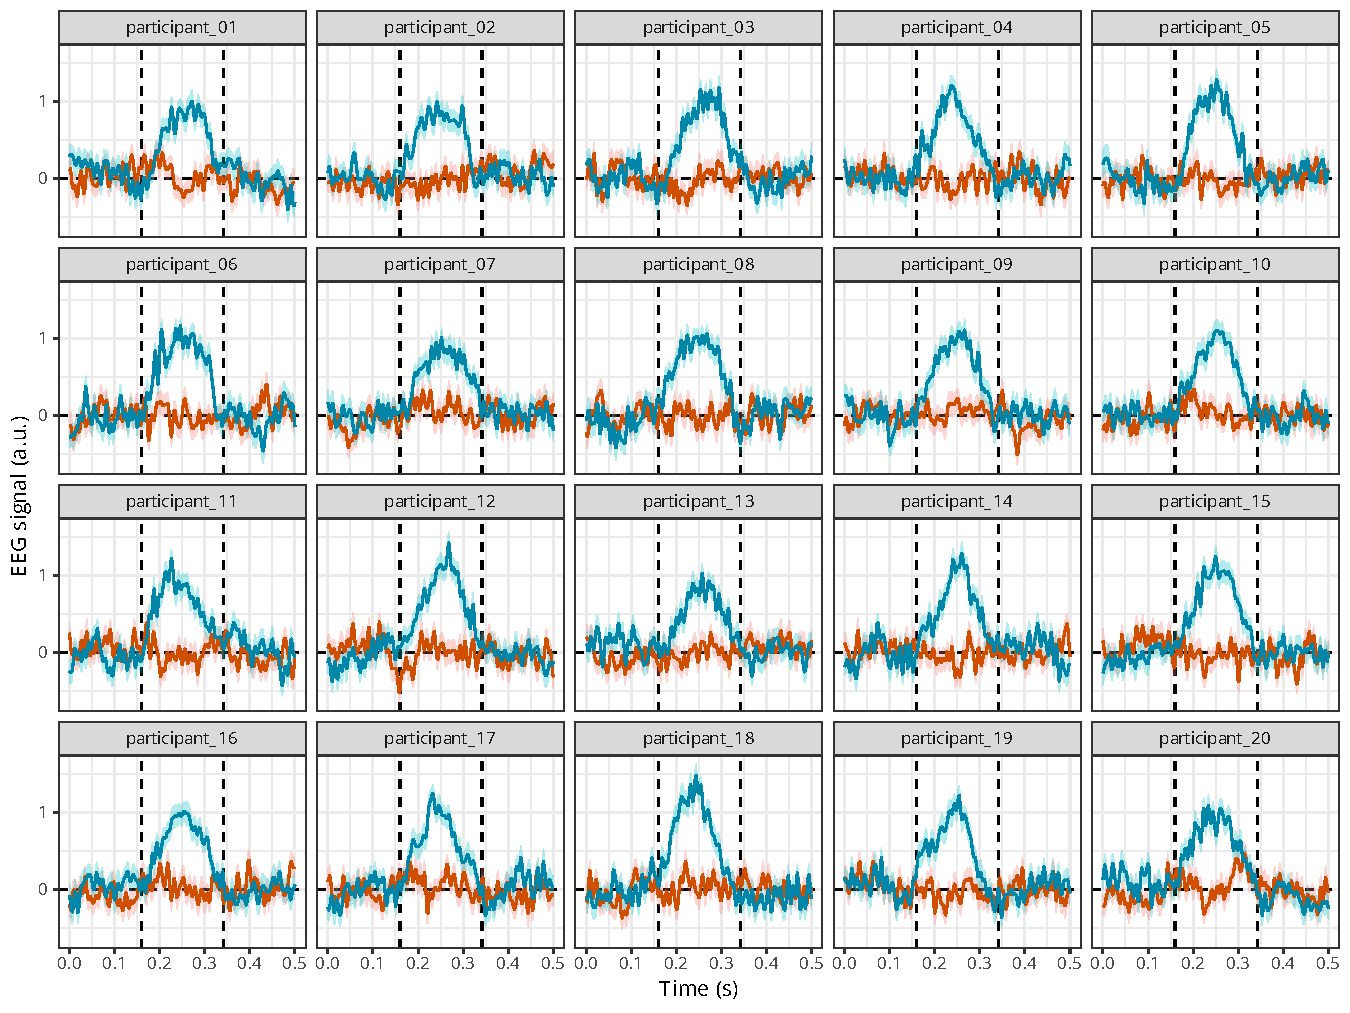
\includegraphics[width=1\textwidth,height=\textheight]{brms_meeg_files/figure-pdf/fig-eeg-1.pdf}

}

\end{figure}%

We computed the average of the ERP difference
(Figure~\ref{fig-erp})\ldots{}

\begin{figure}[!htb]

\caption{\label{fig-erp}Group-level average difference between
conditions (mean +/- standard error of the mean). The `true' onset and
offset are indicated by the vertical dashed lines.}

\centering{

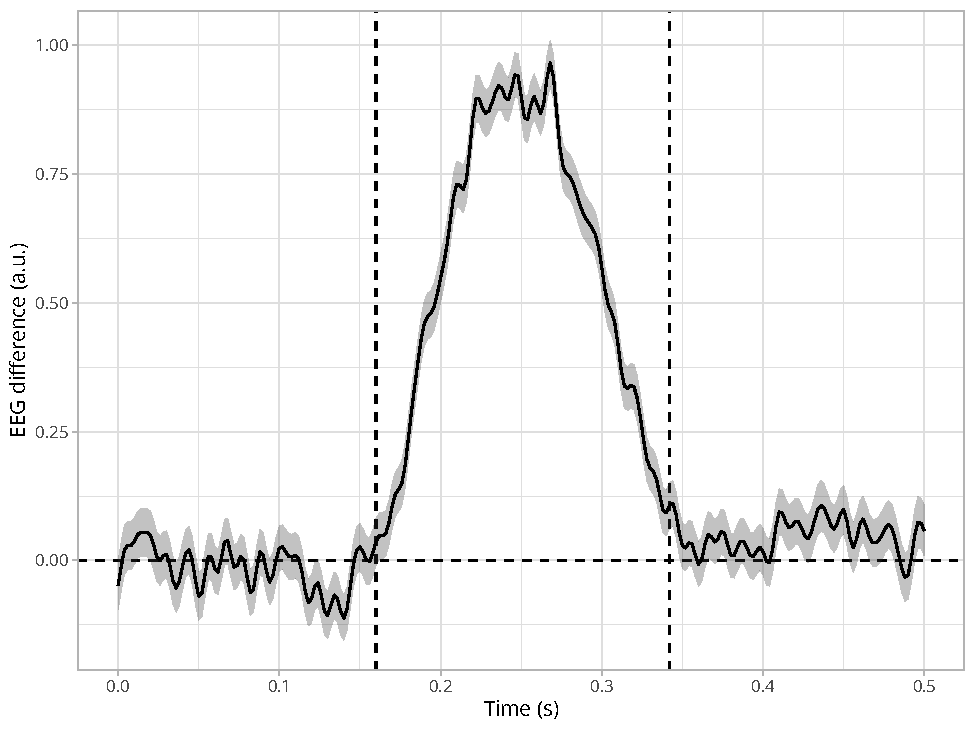
\includegraphics[width=0.75\textwidth,height=\textheight]{brms_meeg_files/figure-pdf/fig-erp-1.pdf}

}

\end{figure}%

\subsection{Model fitting}\label{model-fitting}

We then fitted a GAM and GP regression model using the \texttt{brms}
package (\citeproc{ref-brms2017}{Bürkner, 2017},
\citeproc{ref-brms2018}{2018}; \citeproc{ref-nalborczyk2019}{Nalborczyk
et al., 2019}). We used the default priors in \texttt{brms}, that is,
weakly informative priors. Four Markov Chain Monte-Carlo (MCMC) were ran
for each model to approximate the posterior distribution, including each
5000 iterations and a warmup of 2000 iterations. Posterior convergence
was assessed examining trace plots as well as the Gelman--Rubin statisti
\(\hat{R}\).

\begin{Shaded}
\begin{Highlighting}[]
\CommentTok{\# averaging across participants}
\NormalTok{ppt\_df }\OtherTok{\textless{}{-}}\NormalTok{ raw\_df }\SpecialCharTok{\%\textgreater{}\%}
    \FunctionTok{group\_by}\NormalTok{(participant, condition, time) }\SpecialCharTok{\%\textgreater{}\%}
    \FunctionTok{summarise}\NormalTok{(}\AttributeTok{eeg =} \FunctionTok{mean}\NormalTok{(eeg) ) }\SpecialCharTok{\%\textgreater{}\%}
    \CommentTok{\# mutate(eeg = as.numeric(scale(x = eeg, scale = FALSE) ) ) \%\textgreater{}\%}
    \FunctionTok{ungroup}\NormalTok{()}

\CommentTok{\# defining a contrast for condition}
\FunctionTok{contrasts}\NormalTok{(ppt\_df}\SpecialCharTok{$}\NormalTok{condition) }\OtherTok{\textless{}{-}} \FunctionTok{c}\NormalTok{(}\SpecialCharTok{{-}}\FloatTok{0.5}\NormalTok{, }\FloatTok{0.5}\NormalTok{)}

\CommentTok{\# fitting the GAM}
\NormalTok{gam }\OtherTok{\textless{}{-}} \FunctionTok{brm}\NormalTok{(}
    \CommentTok{\# cubic regression splines with k{-}1 basis functions}
\NormalTok{    eeg }\SpecialCharTok{\textasciitilde{}}\NormalTok{ condition }\SpecialCharTok{+} \FunctionTok{s}\NormalTok{(time, }\AttributeTok{bs =} \StringTok{"cr"}\NormalTok{, }\AttributeTok{k =} \DecValTok{10}\NormalTok{, }\AttributeTok{by =}\NormalTok{ condition),}
    \AttributeTok{data =}\NormalTok{ ppt\_df,}
    \AttributeTok{family =} \FunctionTok{gaussian}\NormalTok{(),}
    \AttributeTok{warmup =} \DecValTok{2000}\NormalTok{,}
    \AttributeTok{iter =} \DecValTok{5000}\NormalTok{,}
    \AttributeTok{chains =} \DecValTok{4}\NormalTok{,}
    \AttributeTok{cores =} \DecValTok{4}\NormalTok{,}
    \AttributeTok{file =} \StringTok{"models/gam.rds"}
\NormalTok{    )}
\end{Highlighting}
\end{Shaded}

Now we fit the GP regression model\ldots{}

\begin{Shaded}
\begin{Highlighting}[]
\CommentTok{\# computing eeg\_diff and averaging across participants}
\CommentTok{\# group\_df \textless{}{-} raw\_df \%\textgreater{}\%}
\CommentTok{\#     group\_by(participant, time) \%\textgreater{}\%}
\CommentTok{\#     pivot\_wider(names\_from = condition, values\_from = eeg, values\_fn = mean) \%\textgreater{}\%}
\CommentTok{\#     mutate(eeg\_diff = cond2 {-} cond1) \%\textgreater{}\%}
\CommentTok{\#     summarise(eeg\_diff = mean(eeg\_diff) ) \%\textgreater{}\%}
\CommentTok{\#     ungroup()}

\CommentTok{\# see https://betanalpha.github.io/assets/case\_studies/gp\_part3/part3.html}
\CommentTok{\# and https://betanalpha.github.io/assets/case\_studies/gaussian\_processes.html}
\NormalTok{gp\_priors }\OtherTok{\textless{}{-}} \FunctionTok{c}\NormalTok{(}
    \FunctionTok{set\_prior}\NormalTok{(}\StringTok{"normal(0, 1)"}\NormalTok{, }\AttributeTok{class =} \StringTok{"Intercept"}\NormalTok{),}
    \FunctionTok{set\_prior}\NormalTok{(}\StringTok{"normal(0, 1)"}\NormalTok{, }\AttributeTok{class =} \StringTok{"b"}\NormalTok{),}
    \FunctionTok{set\_prior}\NormalTok{(}\StringTok{"exponential(1)"}\NormalTok{, }\AttributeTok{class =} \StringTok{"sigma"}\NormalTok{),}
    \FunctionTok{set\_prior}\NormalTok{(}\StringTok{"exponential(1)"}\NormalTok{, }\AttributeTok{class =} \StringTok{"sdgp"}\NormalTok{)}
\NormalTok{    )}

\NormalTok{gp\_model }\OtherTok{\textless{}{-}} \FunctionTok{brm}\NormalTok{(}
    \CommentTok{\# k refers to the number of basis functions for}
    \CommentTok{\# computing Hilbert{-}space approximate GPs}
    \CommentTok{\# if k = NA (default), exact GPs are computed}
    \CommentTok{\# eeg \textasciitilde{} gp(time, by = condition),}
\NormalTok{    eeg }\SpecialCharTok{\textasciitilde{}}\NormalTok{ condition }\SpecialCharTok{+} \FunctionTok{gp}\NormalTok{(time, }\AttributeTok{by =}\NormalTok{ condition, }\AttributeTok{k =} \DecValTok{20}\NormalTok{, }\AttributeTok{cov =} \StringTok{"exp\_quad"}\NormalTok{),}
    \AttributeTok{data =}\NormalTok{ ppt\_df,}
    \AttributeTok{family =} \FunctionTok{gaussian}\NormalTok{(),}
    \CommentTok{\# prior = gp\_priors,}
    \AttributeTok{control =} \FunctionTok{list}\NormalTok{(}\AttributeTok{adapt\_delta =} \FloatTok{0.99}\NormalTok{, }\AttributeTok{max\_treedepth =} \DecValTok{15}\NormalTok{),}
    \AttributeTok{backend =} \StringTok{"cmdstanr"}\NormalTok{,}
    \AttributeTok{iter =} \DecValTok{2000}\NormalTok{,}
    \AttributeTok{chains =} \DecValTok{4}\NormalTok{,}
    \AttributeTok{cores =} \DecValTok{4}\NormalTok{,}
    \AttributeTok{file =} \StringTok{"models/gp.rds"}
\NormalTok{    )}
\end{Highlighting}
\end{Shaded}

And we plot the posterior predictions\ldots{}

\begin{Shaded}
\begin{Highlighting}[]
\CommentTok{\# plotting the posterior predictions}
\FunctionTok{plot\_post\_preds}\NormalTok{(}\AttributeTok{model =}\NormalTok{ gam) }\SpecialCharTok{+} \FunctionTok{plot\_post\_preds}\NormalTok{(}\AttributeTok{model =}\NormalTok{ gp\_model)}
\end{Highlighting}
\end{Shaded}

\begin{figure}[H]

\caption{Posterior predictions of the GAM (left) and GP (right) models.}

{\centering 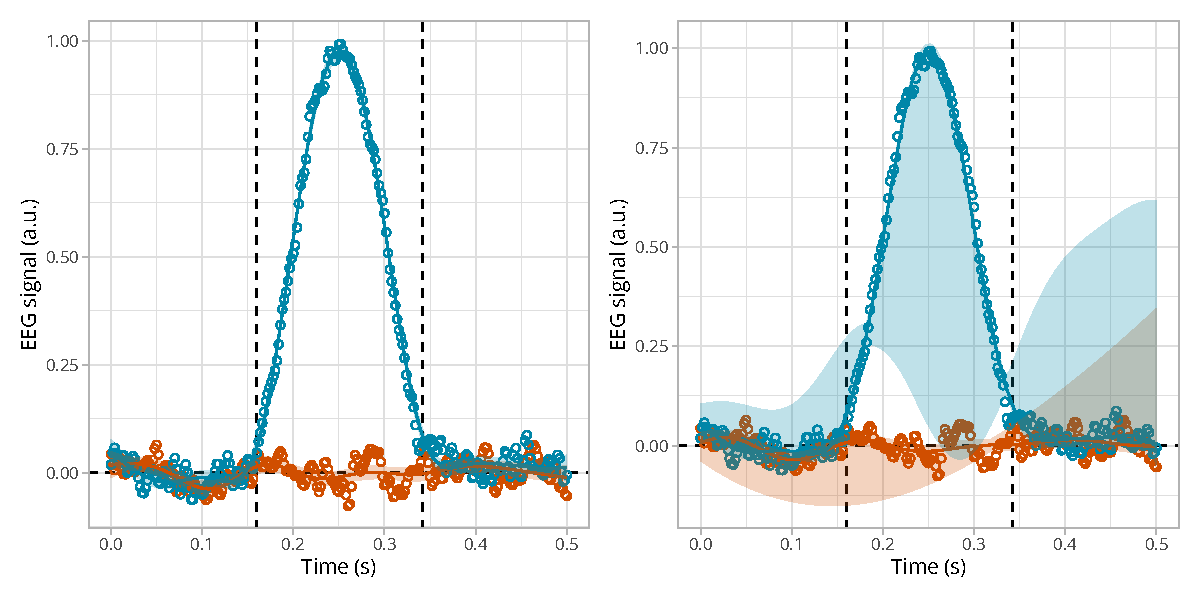
\includegraphics[width=1\textwidth,height=\textheight]{brms_meeg_files/figure-pdf/gam-gp-preds-1.pdf}

}

\end{figure}%

\subsection{Posterior probability of difference above
0}\label{posterior-probability-of-difference-above-0}

We can retrieve the posterior probability of the slope for
\texttt{condition} at each timestep (Figure~\ref{fig-plot-post-slope}).

\begin{figure}[!htb]

\caption{\label{fig-plot-post-slope}Slope for the difference between
conditions according to the GAM (left) or the GP (right).}

\centering{

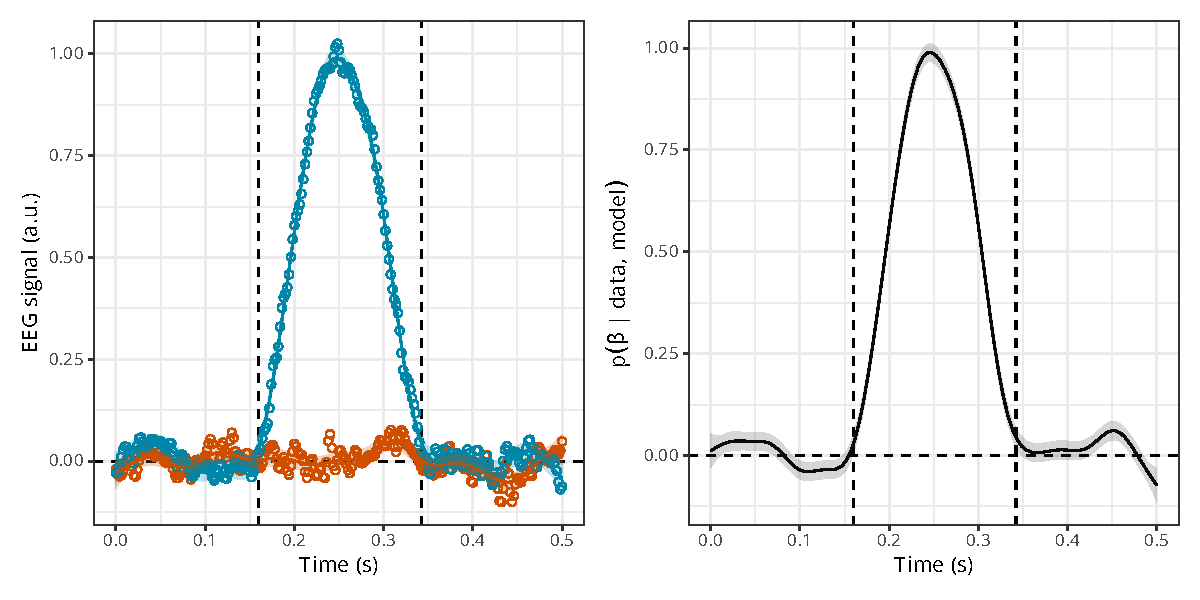
\includegraphics[width=1\textwidth,height=\textheight]{brms_meeg_files/figure-pdf/fig-plot-post-slope-1.pdf}

}

\end{figure}%

We can also compute the posterior probability of the slope for
\texttt{condition} being above \(0+\epsilon\)
(Figure~\ref{fig-post-prob-test}), with \(\epsilon\) defined as 10\% of
the standard deviation of the raw EEG signal.

\begin{figure}[!htb]

\caption{\label{fig-post-prob-test}Posterior probability of the ERP
difference (slope) being above 0 according to the GAM (left) and the GP
(right).}

\centering{

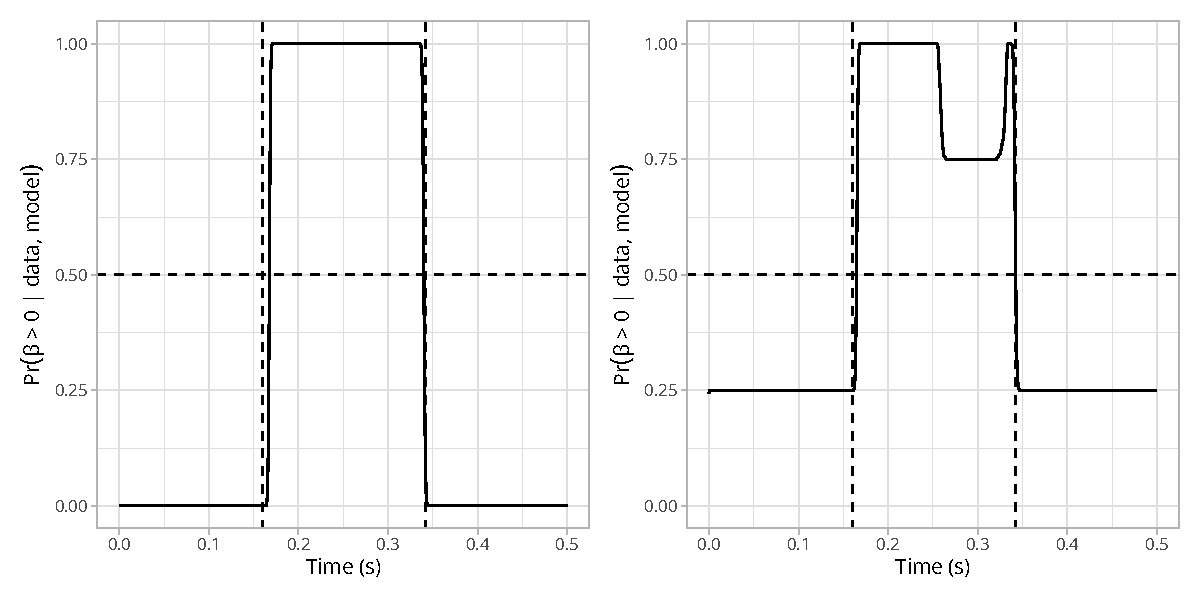
\includegraphics[width=1\textwidth,height=\textheight]{brms_meeg_files/figure-pdf/fig-post-prob-test-1.pdf}

}

\end{figure}%

We can also express this as the ratio of posterior probabilities (i.e.,
\(p/(1-p)\)) and visualise the timecourse of this ratio superimposed
with the conventional thresholds on evidence ratios
(Figure~\ref{fig-post-prob-ratio}).

\begin{figure}[!htb]

\caption{\label{fig-post-prob-ratio}Ratio of posterior probability
according to the GAM. Timesteps above threshold (10) are highlighted in
green.}

\centering{

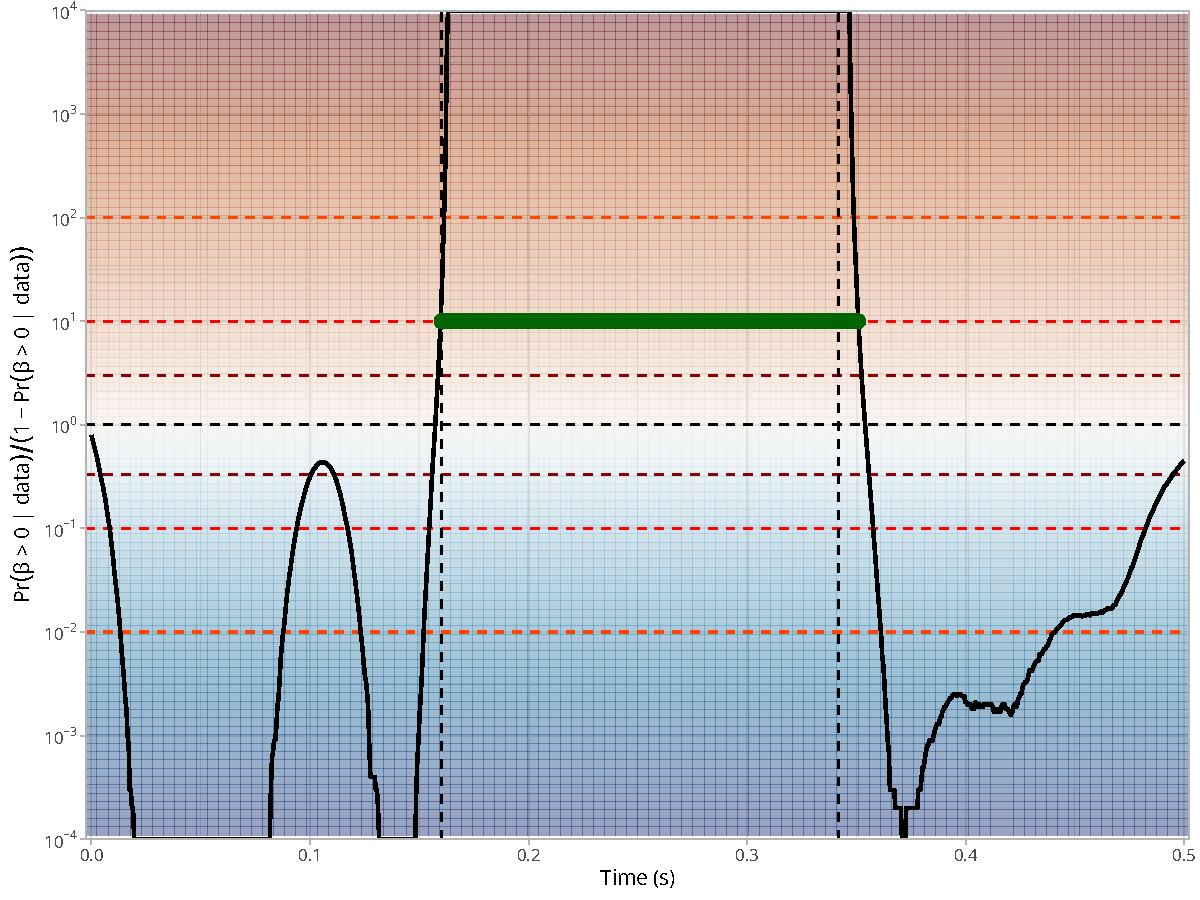
\includegraphics[width=1\textwidth,height=\textheight]{brms_meeg_files/figure-pdf/fig-post-prob-ratio-1.pdf}

}

\end{figure}%

\newpage

\subsection{Multilevel modelling using ERP summary
statistics}\label{multilevel-modelling-using-erp-summary-statistics}

Next we fit a hierarchical/multilevel GAM using summary statistics of
ERPs (mean and SD) at the participant level (similar to what is done in
meta-analysis).

\begin{Shaded}
\begin{Highlighting}[]
\CommentTok{\# averaging across participants}
\NormalTok{summary\_df }\OtherTok{\textless{}{-}}\NormalTok{ raw\_df }\SpecialCharTok{\%\textgreater{}\%}
    \FunctionTok{summarise}\NormalTok{(}
        \AttributeTok{eeg\_mean =} \FunctionTok{mean}\NormalTok{(eeg),}
        \AttributeTok{eeg\_sd =} \FunctionTok{sd}\NormalTok{(eeg),}
        \AttributeTok{.by =} \FunctionTok{c}\NormalTok{(participant, condition, time)}
\NormalTok{        )}

\CommentTok{\# defining a contrast for condition}
\FunctionTok{contrasts}\NormalTok{(summary\_df}\SpecialCharTok{$}\NormalTok{condition) }\OtherTok{\textless{}{-}} \FunctionTok{c}\NormalTok{(}\SpecialCharTok{{-}}\FloatTok{0.5}\NormalTok{, }\FloatTok{0.5}\NormalTok{)}

\CommentTok{\# fitting the GAM}
\NormalTok{meta\_gam }\OtherTok{\textless{}{-}} \FunctionTok{brm}\NormalTok{(}
    \CommentTok{\# using by{-}participant SD of ERPs across trials}
\NormalTok{    eeg\_mean }\SpecialCharTok{|} \FunctionTok{se}\NormalTok{(eeg\_sd) }\SpecialCharTok{\textasciitilde{}}
\NormalTok{        condition }\SpecialCharTok{+} \FunctionTok{s}\NormalTok{(time, }\AttributeTok{bs =} \StringTok{"cr"}\NormalTok{, }\AttributeTok{k =} \DecValTok{10}\NormalTok{, }\AttributeTok{by =}\NormalTok{ condition) }\SpecialCharTok{+}
\NormalTok{        (}\DecValTok{1} \SpecialCharTok{|}\NormalTok{ participant),}
    \AttributeTok{data =}\NormalTok{ summary\_df,}
    \AttributeTok{family =} \FunctionTok{gaussian}\NormalTok{(),}
    \AttributeTok{warmup =} \DecValTok{2000}\NormalTok{,}
    \AttributeTok{iter =} \DecValTok{5000}\NormalTok{,}
    \AttributeTok{chains =} \DecValTok{4}\NormalTok{,}
    \AttributeTok{cores =} \DecValTok{4}\NormalTok{,}
    \AttributeTok{file =} \StringTok{"models/meta\_gam.rds"}
\NormalTok{    )}
\end{Highlighting}
\end{Shaded}

\begin{Shaded}
\begin{Highlighting}[]
\CommentTok{\# fitting the GP}
\NormalTok{meta\_gp }\OtherTok{\textless{}{-}} \FunctionTok{brm}\NormalTok{(}
    \CommentTok{\# using by{-}participant SD of ERPs across trials}
\NormalTok{    eeg\_mean }\SpecialCharTok{|} \FunctionTok{se}\NormalTok{(eeg\_sd) }\SpecialCharTok{\textasciitilde{}}
\NormalTok{        condition }\SpecialCharTok{+} \FunctionTok{gp}\NormalTok{(time, }\AttributeTok{k =} \DecValTok{20}\NormalTok{, }\AttributeTok{by =}\NormalTok{ condition) }\SpecialCharTok{+}
\NormalTok{        (}\DecValTok{1} \SpecialCharTok{|}\NormalTok{ participant),}
    \AttributeTok{data =}\NormalTok{ summary\_df,}
    \AttributeTok{family =} \FunctionTok{gaussian}\NormalTok{(),}
    \AttributeTok{control =} \FunctionTok{list}\NormalTok{(}\AttributeTok{adapt\_delta =} \FloatTok{0.99}\NormalTok{),}
    \AttributeTok{iter =} \DecValTok{5000}\NormalTok{,}
    \AttributeTok{chains =} \DecValTok{4}\NormalTok{,}
    \AttributeTok{cores =} \DecValTok{4}\NormalTok{,}
    \AttributeTok{file =} \StringTok{"models/meta\_gp.rds"}
\NormalTok{    )}
\end{Highlighting}
\end{Shaded}

\begin{Shaded}
\begin{Highlighting}[]
\CommentTok{\# plotting the posterior predictions}
\NormalTok{meta\_gam\_preds }\OtherTok{\textless{}{-}} \FunctionTok{plot}\NormalTok{(}
    \FunctionTok{conditional\_effects}\NormalTok{(}\AttributeTok{x =}\NormalTok{ meta\_gam, }\AttributeTok{effect =} \StringTok{"time:condition"}\NormalTok{),}
    \AttributeTok{points =} \ConstantTok{FALSE}\NormalTok{, }\AttributeTok{theme =} \FunctionTok{theme\_light}\NormalTok{(), }\AttributeTok{plot =} \ConstantTok{FALSE}
\NormalTok{    )[[}\DecValTok{1}\NormalTok{]] }\SpecialCharTok{+}
    \FunctionTok{scale\_colour\_met\_d}\NormalTok{(}\AttributeTok{name =} \StringTok{"Johnson"}\NormalTok{) }\SpecialCharTok{+}
    \FunctionTok{scale\_fill\_met\_d}\NormalTok{(}\AttributeTok{name =} \StringTok{"Johnson"}\NormalTok{) }\SpecialCharTok{+}
    \FunctionTok{labs}\NormalTok{(}\AttributeTok{x =} \StringTok{"Time (s)"}\NormalTok{, }\AttributeTok{y =} \StringTok{"EEG signal (a.u.)"}\NormalTok{)}
\NormalTok{meta\_gp\_preds }\OtherTok{\textless{}{-}} \FunctionTok{plot}\NormalTok{(}
    \FunctionTok{conditional\_effects}\NormalTok{(}\AttributeTok{x =}\NormalTok{ meta\_gp, }\AttributeTok{effect =} \StringTok{"time:condition"}\NormalTok{),}
    \AttributeTok{points =} \ConstantTok{FALSE}\NormalTok{, }\AttributeTok{theme =} \FunctionTok{theme\_light}\NormalTok{(), }\AttributeTok{plot =} \ConstantTok{FALSE}
\NormalTok{    )[[}\DecValTok{1}\NormalTok{]] }\SpecialCharTok{+}
    \FunctionTok{scale\_colour\_met\_d}\NormalTok{(}\AttributeTok{name =} \StringTok{"Johnson"}\NormalTok{) }\SpecialCharTok{+}
    \FunctionTok{scale\_fill\_met\_d}\NormalTok{(}\AttributeTok{name =} \StringTok{"Johnson"}\NormalTok{) }\SpecialCharTok{+}
    \FunctionTok{labs}\NormalTok{(}\AttributeTok{x =} \StringTok{"Time (s)"}\NormalTok{, }\AttributeTok{y =} \StringTok{"EEG signal (a.u.)"}\NormalTok{)}

\CommentTok{\# combining the two plots}
\NormalTok{meta\_gam\_preds }\SpecialCharTok{+}\NormalTok{ meta\_gp\_preds}
\end{Highlighting}
\end{Shaded}

\begin{figure}[H]

\caption{Posterior predictions for the hierarchical GAM and GP.}

{\centering 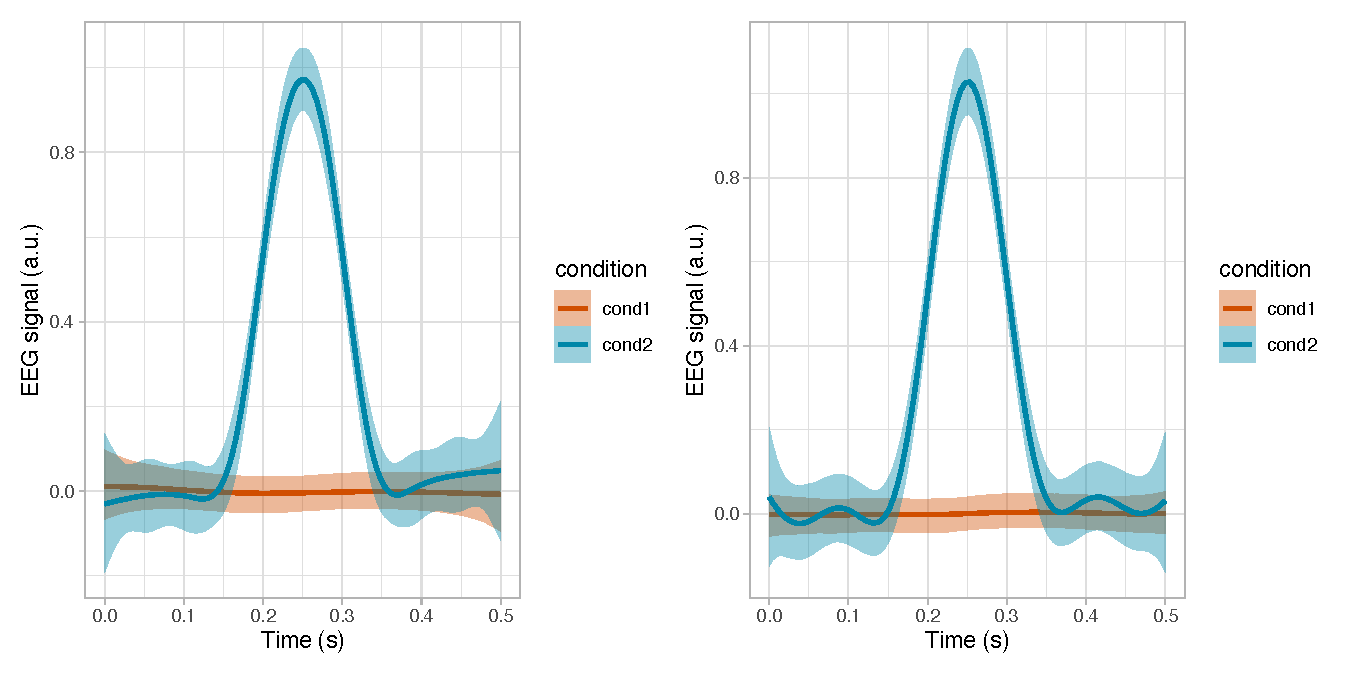
\includegraphics[width=1\textwidth,height=\textheight]{brms_meeg_files/figure-pdf/meta-gp-preds-1.pdf}

}

\end{figure}%

\newpage

\subsection{Error properties of the proposed
approach}\label{error-properties-of-the-proposed-approach}

We then computed the difference between the true and estimated
onset/offset of the ERP difference
(\(\text{error}:=|\hat{\theta}-\theta|\)), according to various
\texttt{eps} and \texttt{threshold} values. Remember that the signal is
generated from a truncated Gaussian with an objective onset at 160 ms, a
maximum at 250 ms, and an offset at 342 ms. Figure~\ref{fig-onset-error}
shows that the hierarchical GAM can \emph{exactly} recover the true
onset and offset values, given some reasonable choice of \texttt{eps}
and \texttt{threshold} values (e.g., a threshold of 20).

\begin{verbatim}
   eps threshold estimated_onset estimated_offset error_onset error_offset
1 0.00        13            0.16             0.34           0        0.002
2 0.00        14            0.16             0.34           0        0.002
3 0.00        15            0.16             0.34           0        0.002
4 0.00        16            0.16             0.34           0        0.002
5 0.00        17            0.16             0.34           0        0.002
6 0.01        10            0.16             0.34           0        0.002
\end{verbatim}

\begin{figure}[!htb]

\caption{\label{fig-onset-error}Error function of onset (left) and
offset (right) estimation according to various eps and threshold values
(according to the hierarchical GAM). Minimum error values are indicated
by red crosses.}

\centering{

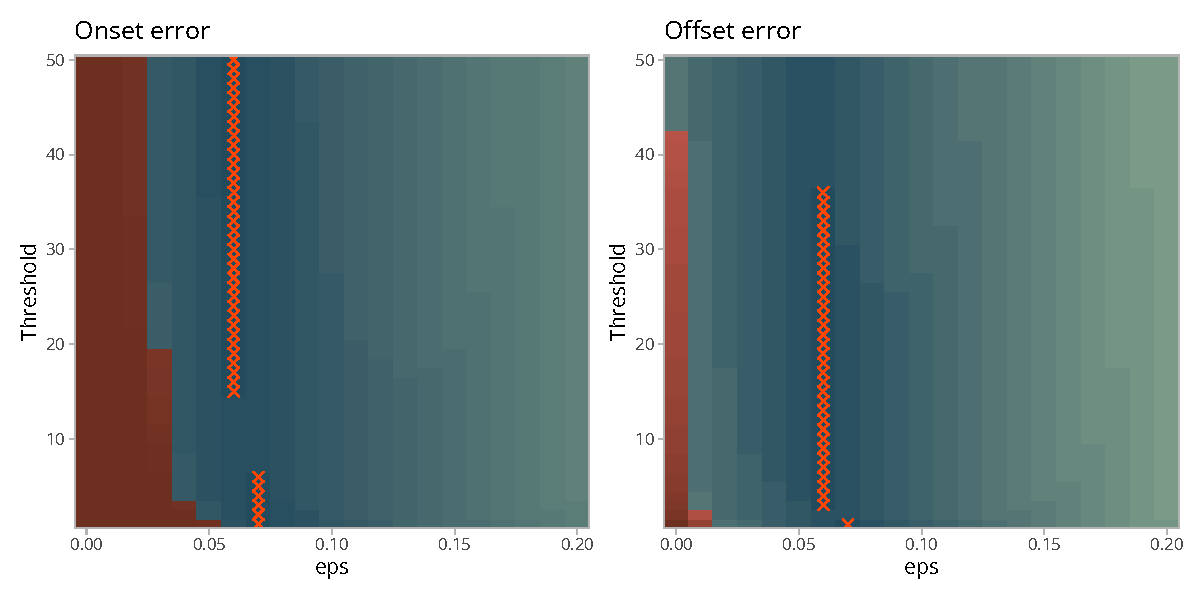
\includegraphics[width=1\textwidth,height=\textheight]{brms_meeg_files/figure-pdf/fig-onset-error-1.pdf}

}

\end{figure}%

\newpage

\subsection{Application to actual M/EEG
data}\label{application-to-actual-meeg-data}

Assessing the reliability of the proposed approach (in comparison to
other methods) using some sort of split-half reliability
(\citeproc{ref-rosenblatt2018}{Rosenblatt et al., 2018})?

\subsection{Comparing the identified onsets/offsets to other
approaches}\label{comparing-the-identified-onsetsoffsets-to-other-approaches}

We considered five methods for multiplicity corrections: two FDR
methods; two cluster-based methods; and the maximum statistics. The two
FDR methods were BH95 (Benjamini \& Hochberg, 1995;
10.1111/j.2517-6161.1995.tb02031.x) and BY01 (Benjamini \& Yekutieli,
2001; 10.1214/aos/1013699998), which were applied to the permutation
p-values using the \texttt{p.adjust} function in \texttt{R}. The first
cluster-based inference was implemented using a cluster-sum statistic of
squared t-values\ldots{}

We also compared the performance of the GAMM (in correctly
identifying/estimating the onset and offset of ERP difference across
conditions) to the performance of the binary segmentation method as
implemented in the \texttt{R} package \texttt{changepoint} v 2.2.4
(\citeproc{ref-changepoint}{Killick et al., 2022a}), threshold-free
cluster enhancement (TFCE, \citeproc{ref-smith2009}{Smith \& Nichols,
2009}), as implemented in \texttt{MNE-Python}
(\citeproc{ref-gramfort2013}{Gramfort, 2013}), and using the raw t-, p-,
or s-values timecourse. S-values
(\citeproc{ref-greenland2019}{Greenland, 2019})\ldots{}

\begin{figure}[H]

\caption{Timecourse of squared t-values and s-values (continuous measure
of evidence given by -log2(p-value)) with true onset and onset
identified using the raw (uncorrected) p-values or the corrected
p-values (BH, BY, Holm).}

{\centering 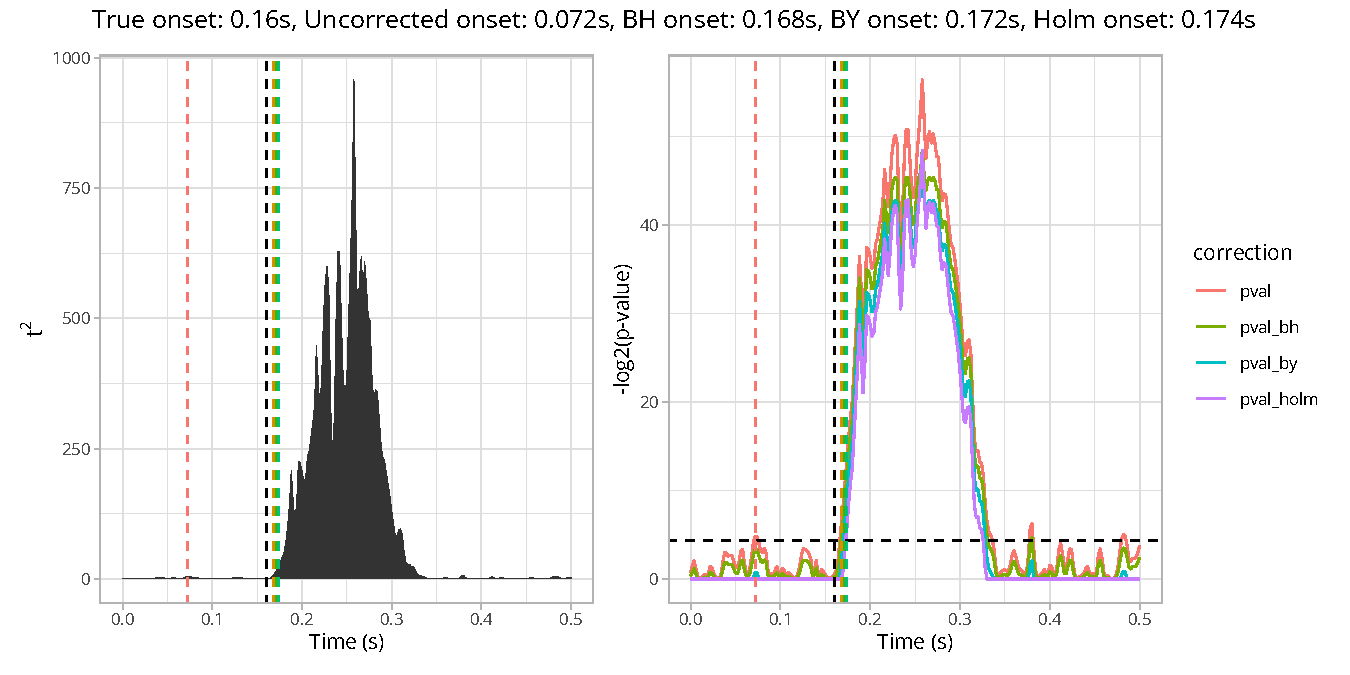
\includegraphics[width=1\textwidth,height=\textheight]{brms_meeg_files/figure-pdf/test-1d-1.pdf}

}

\end{figure}%

\begin{figure}[H]

\caption{T-values timecourse with true onset/offset and onset/offset
identified using the changepoint package (binary segmentation method, in
green).}

{\centering 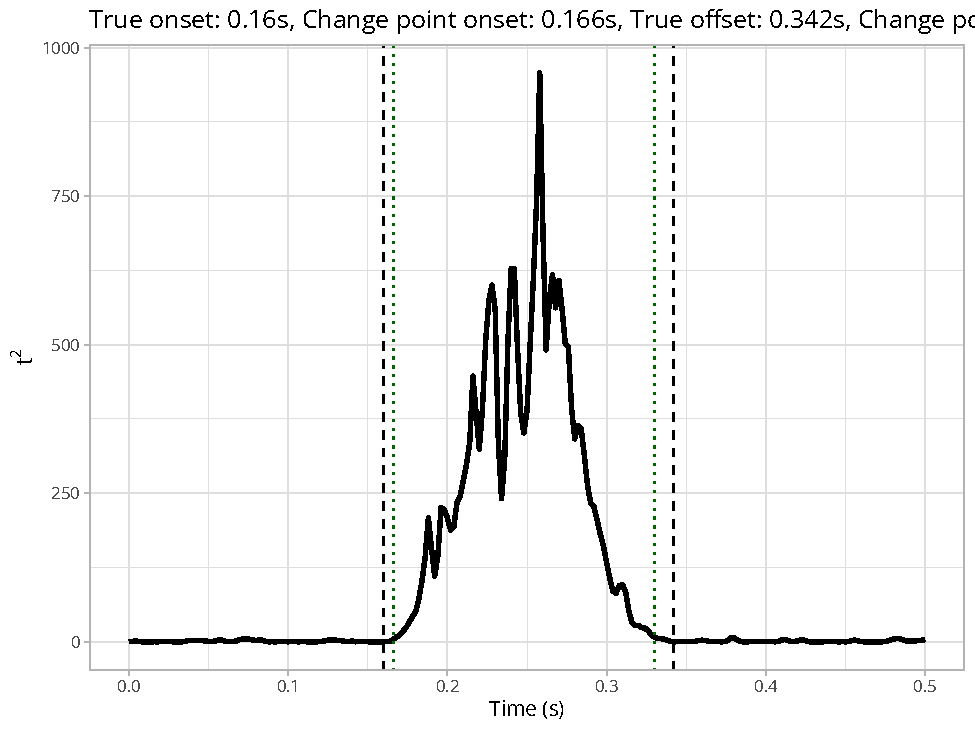
\includegraphics[width=0.75\textwidth,height=\textheight]{brms_meeg_files/figure-pdf/changepoint-1.pdf}

}

\end{figure}%

Now cluster-based permutations using \texttt{MNE-Python}
(\citeproc{ref-gramfort2013}{Gramfort, 2013}) via the \texttt{R} package
\texttt{reticulate} v 1.35.0 (\citeproc{ref-reticulate}{Ushey et al.,
2024})\ldots{}

\begin{Shaded}
\begin{Highlighting}[]
\CommentTok{\# importing the decoding scores}
\NormalTok{p\_values\_df }\OtherTok{\textless{}{-}} \FunctionTok{readRDS}\NormalTok{(}\AttributeTok{file =} \StringTok{"results/mne\_permutation\_decoding\_scores.rds"}\NormalTok{)}

\CommentTok{\# plotting the s{-}values ({-}log2(p{-}values))}
\NormalTok{p\_values\_df }\SpecialCharTok{\%\textgreater{}\%}
    \FunctionTok{mutate}\NormalTok{(}\AttributeTok{sval =} \SpecialCharTok{{-}}\FunctionTok{log2}\NormalTok{(pval) ) }\SpecialCharTok{\%\textgreater{}\%}
    \FunctionTok{ggplot}\NormalTok{(}\FunctionTok{aes}\NormalTok{(}\AttributeTok{x =}\NormalTok{ time, }\AttributeTok{y =}\NormalTok{ sval) ) }\SpecialCharTok{+}
    \FunctionTok{geom\_line}\NormalTok{(}\AttributeTok{linewidth =} \FloatTok{0.5}\NormalTok{) }\SpecialCharTok{+}
    \FunctionTok{geom\_hline}\NormalTok{(}\AttributeTok{yintercept =} \SpecialCharTok{{-}}\FunctionTok{log2}\NormalTok{(}\FloatTok{0.05}\NormalTok{), }\AttributeTok{linetype =} \DecValTok{2}\NormalTok{) }\SpecialCharTok{+}
    \FunctionTok{labs}\NormalTok{(}
        \AttributeTok{x =} \StringTok{"Time (s)"}\NormalTok{,}
        \AttributeTok{y =} \StringTok{"{-}log2(p{-}value)"}
\NormalTok{        )}
\end{Highlighting}
\end{Shaded}

\begin{figure}[!htb]

\caption{\label{fig-mne-cluster}Cluster-based permutation tests via
MNE-Python.}

\centering{

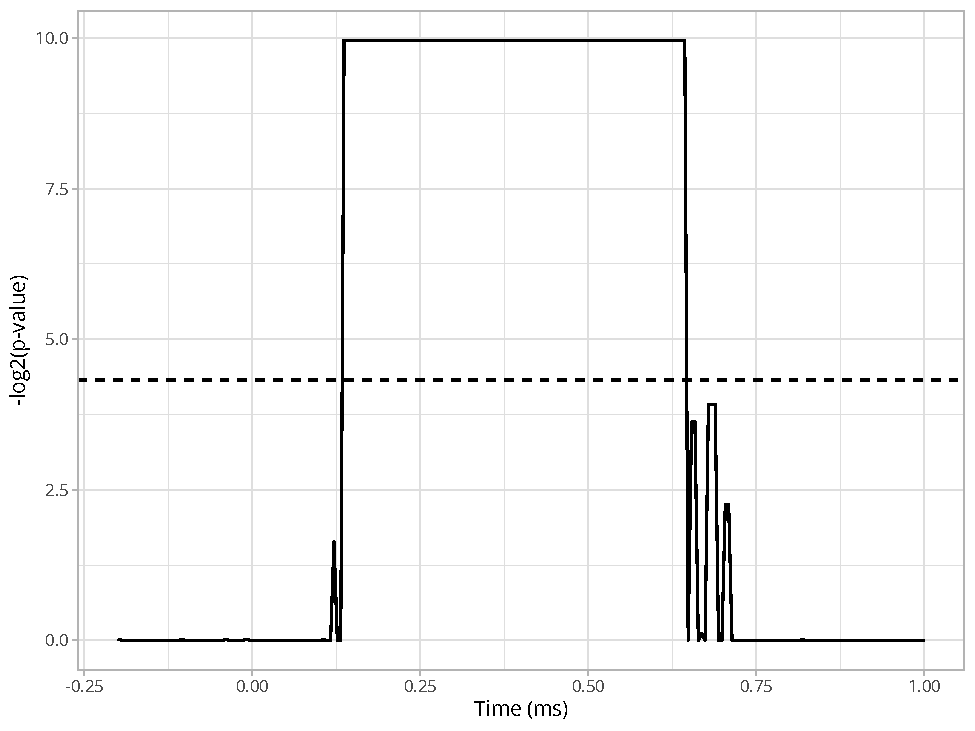
\includegraphics[width=0.75\textwidth,height=\textheight]{brms_meeg_files/figure-pdf/fig-mne-cluster-1.pdf}

}

\end{figure}%

\subsection{Simulation study}\label{simulation-study}

Onset/offset estimation methods were assessed using these summary
statistics of the Monte Carlo sampling distributions of onsets: bias
(median-based), mean absolute error (MAE) and variance, with 10.000
iterations (i.e., 10.000 simulated datasets)\ldots{}

\newpage

\section{Results}\label{results}

\ldots{}

\newpage

\section{Discussion}\label{discussion}

\ldots{}

\subsection{Summary of the proposed
approach}\label{summary-of-the-proposed-approach}

\ldots{}

\subsection{Increasing potential
usage}\label{increasing-potential-usage}

Prepare a wrapper \texttt{R} package and show how to call it in
\texttt{Python} and integrate it with \texttt{MNE-Python}
(\citeproc{ref-gramfort2013}{Gramfort, 2013}) pipelines\ldots{}

\subsection{Limitations and future
directions}\label{limitations-and-future-directions}

Can be applied to any 1D timeseries (e.g., pupillometry,
electromyography)\ldots{} Extending the approach to spatiotemporal data
(i.e., time + sensors)\ldots{}

\subsection{Conclusions}\label{conclusions}

\ldots{}

\newpage

\section{Packages}\label{packages}

We used R version 4.2.3 (\citeproc{ref-base}{R Core Team, 2023}) and the
following R packages: brms v. 2.22.0 (\citeproc{ref-brms2017}{Bürkner,
2017}, \citeproc{ref-brms2018}{2018}, \citeproc{ref-brms2021}{2021}),
changepoint v. 2.2.4 (\citeproc{ref-changepoint2022}{Killick et al.,
2022b}; \citeproc{ref-changepoint2014}{Killick \& Eckley, 2014}),
grateful v. 0.2.10 (\citeproc{ref-grateful}{Rodriguez-Sanchez \&
Jackson, 2023}), knitr v. 1.45 (\citeproc{ref-knitr2014}{Xie, 2014},
\citeproc{ref-knitr2015}{2015}, \citeproc{ref-knitr2023}{2023}),
MetBrewer v. 0.2.0 (\citeproc{ref-MetBrewer}{Mills, 2022}), pakret v.
0.2.2 (\citeproc{ref-pakret}{Gallou, 2024}), patchwork v. 1.2.0
(\citeproc{ref-patchwork}{T. L. Pedersen, 2024}), rmarkdown v. 2.29
(\citeproc{ref-rmarkdown2024}{Allaire et al., 2024};
\citeproc{ref-rmarkdown2018}{Xie et al., 2018},
\citeproc{ref-rmarkdown2020}{2020}), scales v. 1.3.0
(\citeproc{ref-scales}{Wickham et al., 2023}), scico v. 1.5.0
(\citeproc{ref-scico}{T. L. Pedersen \& Crameri, 2023}), tidybayes v.
3.0.6 (\citeproc{ref-tidybayes}{Kay, 2023}), tidyverse v. 2.0.0
(\citeproc{ref-tidyverse}{Wickham et al., 2019}).

\newpage

\section{References}\label{references}

\phantomsection\label{refs}
\begin{CSLReferences}{1}{0}
\bibitem[\citeproctext]{ref-abugaber2023}
Abugaber, D., Finestrat, I., Luque, A., \& Morgan-Short, K. (2023).
Generalized additive mixed modeling of EEG supports dual-route accounts
of morphosyntax in suggesting no word frequency effects on processing of
regular grammatical forms. \emph{Journal of Neurolinguistics},
\emph{67}, 101137.
\url{https://doi.org/10.1016/j.jneuroling.2023.101137}

\bibitem[\citeproctext]{ref-rmarkdown2024}
Allaire, J., Xie, Y., Dervieux, C., McPherson, J., Luraschi, J., Ushey,
K., Atkins, A., Wickham, H., Cheng, J., Chang, W., \& Iannone, R.
(2024). \emph{{rmarkdown}: Dynamic documents for r}.
\url{https://github.com/rstudio/rmarkdown}

\bibitem[\citeproctext]{ref-brms2017}
Bürkner, P.-C. (2017). {brms}: An {R} package for {Bayesian} multilevel
models using {Stan}. \emph{Journal of Statistical Software},
\emph{80}(1), 1--28. \url{https://doi.org/10.18637/jss.v080.i01}

\bibitem[\citeproctext]{ref-brms2018}
Bürkner, P.-C. (2018). Advanced {Bayesian} multilevel modeling with the
{R} package {brms}. \emph{The R Journal}, \emph{10}(1), 395--411.
\url{https://doi.org/10.32614/RJ-2018-017}

\bibitem[\citeproctext]{ref-brms2021}
Bürkner, P.-C. (2021). Bayesian item response modeling in {R} with
{brms} and {Stan}. \emph{Journal of Statistical Software},
\emph{100}(5), 1--54. \url{https://doi.org/10.18637/jss.v100.i05}

\bibitem[\citeproctext]{ref-combrisson_exceeding_2015}
Combrisson, E., \& Jerbi, K. (2015). Exceeding chance level by chance:
{The} caveat of theoretical chance levels in brain signal classification
and statistical assessment of decoding accuracy. \emph{Journal of
Neuroscience Methods}, \emph{250}, 126--136.
\url{https://doi.org/10.1016/j.jneumeth.2015.01.010}

\bibitem[\citeproctext]{ref-dimigen2021}
Dimigen, O., \& Ehinger, B. V. (2021). Regression-based analysis of
combined EEG and eye-tracking data: Theory and applications.
\emph{Journal of Vision}, \emph{21}(1), 3.
\url{https://doi.org/10.1167/jov.21.1.3}

\bibitem[\citeproctext]{ref-dunagan2024}
Dunagan, D., Jordan, T., Hale, J. T., Pylkkänen, L., \& Chacón, D. A.
(2024). \emph{Evaluating the timecourses of morpho-orthographic,
lexical, and grammatical processing following rapid parallel visual
presentation: An EEG investigation in english}.
\url{http://dx.doi.org/10.1101/2024.04.10.588861}

\bibitem[\citeproctext]{ref-ehinger_unfold_2019}
Ehinger, B. V., \& Dimigen, O. (2019). Unfold: An integrated toolbox for
overlap correction, non-linear modeling, and regression-based {EEG}
analysis. \emph{PeerJ}, \emph{7}, e7838.
\url{https://doi.org/10.7717/peerj.7838}

\bibitem[\citeproctext]{ref-eklund2016}
Eklund, A., Nichols, T. E., \& Knutsson, H. (2016). Cluster failure: Why
fMRI inferences for spatial extent have inflated false-positive rates.
\emph{Proceedings of the National Academy of Sciences}, \emph{113}(28),
7900--7905. \url{https://doi.org/10.1073/pnas.1602413113}

\bibitem[\citeproctext]{ref-fischer2013}
Fischer, Adrian~G., \& Ullsperger, M. (2013). Real and Fictive Outcomes
Are Processed Differently but Converge on a Common Adaptive Mechanism.
\emph{Neuron}, \emph{79}(6), 1243--1255.
\url{https://doi.org/10.1016/j.neuron.2013.07.006}

\bibitem[\citeproctext]{ref-frossard2021}
Frossard, J., \& Renaud, O. (2021). Permutation Tests for Regression,
ANOVA, and Comparison of Signals: The {\textbf{permuco}} Package.
\emph{Journal of Statistical Software}, \emph{99}(15).
\url{https://doi.org/10.18637/jss.v099.i15}

\bibitem[\citeproctext]{ref-frossard2022}
Frossard, J., \& Renaud, O. (2022). The cluster depth tests: Toward
point-wise strong control of the family-wise error rate in massively
univariate tests with application to M/EEG. \emph{NeuroImage},
\emph{247}, 118824.
\url{https://doi.org/10.1016/j.neuroimage.2021.118824}

\bibitem[\citeproctext]{ref-pakret}
Gallou, A. (2024). \emph{{pakret}: Cite {``{R}''} packages on the fly in
{``{R Markdown}''} and {``{Quarto}''}}.
\url{https://CRAN.R-project.org/package=pakret}

\bibitem[\citeproctext]{ref-gramfort2013}
Gramfort, A. (2013). MEG and EEG data analysis with MNE-python.
\emph{Frontiers in Neuroscience}, \emph{7}.
\url{https://doi.org/10.3389/fnins.2013.00267}

\bibitem[\citeproctext]{ref-greenland2019}
Greenland, S. (2019). Valid {\emph{P}} -Values Behave Exactly as They
Should: Some Misleading Criticisms of {\emph{P}} -Values and Their
Resolution With {\emph{S}} -Values. \emph{The American Statistician},
\emph{73}(sup1), 106--114.
\url{https://doi.org/10.1080/00031305.2018.1529625}

\bibitem[\citeproctext]{ref-hauk2006}
Hauk, O., Davis, M. H., Ford, M., Pulvermüller, F., \& Marslen-Wilson,
W. D. (2006). The time course of visual word recognition as revealed by
linear regression analysis of ERP data. \emph{NeuroImage}, \emph{30}(4),
1383--1400. \url{https://doi.org/10.1016/j.neuroimage.2005.11.048}

\bibitem[\citeproctext]{ref-hayasaka_validating_2003}
Hayasaka, S. (2003). Validating cluster size inference: Random field and
permutation methods. \emph{NeuroImage}, \emph{20}(4), 2343--2356.
\url{https://doi.org/10.1016/j.neuroimage.2003.08.003}

\bibitem[\citeproctext]{ref-tidybayes}
Kay, M. (2023). \emph{{tidybayes}: Tidy data and geoms for {Bayesian}
models}. \url{https://doi.org/10.5281/zenodo.1308151}

\bibitem[\citeproctext]{ref-changepoint2014}
Killick, R., \& Eckley, I. A. (2014). {changepoint}: An {R} package for
changepoint analysis. \emph{Journal of Statistical Software},
\emph{58}(3), 1--19.
\url{https://www.jstatsoft.org/article/view/v058i03}

\bibitem[\citeproctext]{ref-changepoint}
Killick, R., Haynes, K., \& Eckley, I. A. (2022a). \emph{{changepoint}:
An {R} package for changepoint analysis}.
\url{https://CRAN.R-project.org/package=changepoint}

\bibitem[\citeproctext]{ref-changepoint2022}
Killick, R., Haynes, K., \& Eckley, I. A. (2022b). \emph{{changepoint}:
An {R} package for changepoint analysis}.
\url{https://CRAN.R-project.org/package=changepoint}

\bibitem[\citeproctext]{ref-king2014}
King, J.-R., \& Dehaene, S. (2014). Characterizing the dynamics of
mental representations: the temporal generalization method. \emph{Trends
in Cognitive Sciences}, \emph{18}(4), 203--210.
\url{https://doi.org/10.1016/j.tics.2014.01.002}

\bibitem[\citeproctext]{ref-luck_how_2017}
Luck, S. J., \& Gaspelin, N. (2017). How to get statistically
significant effects in any {ERP} experiment (and why you shouldn't).
\emph{Psychophysiology}, \emph{54}(1), 146--157.
\url{https://doi.org/10.1111/psyp.12639}

\bibitem[\citeproctext]{ref-maris2011}
Maris, E. (2011). Statistical testing in electrophysiological studies.
\emph{Psychophysiology}, \emph{49}(4), 549--565.
\url{https://doi.org/10.1111/j.1469-8986.2011.01320.x}

\bibitem[\citeproctext]{ref-maris2007}
Maris, E., \& Oostenveld, R. (2007). Nonparametric statistical testing
of EEG- and MEG-data. \emph{Journal of Neuroscience Methods},
\emph{164}(1), 177--190.
\url{https://doi.org/10.1016/j.jneumeth.2007.03.024}

\bibitem[\citeproctext]{ref-meulman2015}
Meulman, N., Wieling, M., Sprenger, S. A., Stowe, L. A., \& Schmid, M.
S. (2015). Age Effects in L2 Grammar Processing as Revealed by ERPs and
How (Not) to Study Them. \emph{PLOS ONE}, \emph{10}(12), e0143328.
\url{https://doi.org/10.1371/journal.pone.0143328}

\bibitem[\citeproctext]{ref-MetBrewer}
Mills, B. R. (2022). \emph{{MetBrewer}: Color palettes inspired by works
at the metropolitan museum of art}.
\url{https://CRAN.R-project.org/package=MetBrewer}

\bibitem[\citeproctext]{ref-nalborczyk2019}
Nalborczyk, L., Batailler, C., Lœvenbruck, H., Vilain, A., \& Bürkner,
P.-C. (2019). An Introduction to Bayesian Multilevel Models Using brms:
A Case Study of Gender Effects on Vowel Variability in Standard
Indonesian. \emph{Journal of Speech, Language, and Hearing Research},
\emph{62}(5), 1225--1242.
\url{https://doi.org/10.1044/2018_jslhr-s-18-0006}

\bibitem[\citeproctext]{ref-pedersen_hierarchical_2019}
Pedersen, E. J., Miller, D. L., Simpson, G. L., \& Ross, N. (2019).
Hierarchical generalized additive models in ecology: An introduction
with mgcv. \emph{PeerJ}, \emph{7}, e6876.
\url{https://doi.org/10.7717/peerj.6876}

\bibitem[\citeproctext]{ref-patchwork}
Pedersen, T. L. (2024). \emph{{patchwork}: The composer of plots}.
\url{https://CRAN.R-project.org/package=patchwork}

\bibitem[\citeproctext]{ref-scico}
Pedersen, T. L., \& Crameri, F. (2023). \emph{{scico}: Colour palettes
based on the scientific colour-maps}.
\url{https://CRAN.R-project.org/package=scico}

\bibitem[\citeproctext]{ref-pernet2022}
Pernet, C. (2022). Electroencephalography robust statistical linear
modelling using a single weight per trial. \emph{Aperture Neuro},
\emph{2}, 1--22.
\url{https://doi.org/10.52294/apertureneuro.2022.2.seoo9435}

\bibitem[\citeproctext]{ref-pernet2015}
Pernet, C. R., Latinus, M., Nichols, T. E., \& Rousselet, G. A. (2015).
Cluster-based computational methods for mass univariate analyses of
event-related brain potentials/fields: A simulation study. \emph{Journal
of Neuroscience Methods}, \emph{250}, 85--93.
\url{https://doi.org/10.1016/j.jneumeth.2014.08.003}

\bibitem[\citeproctext]{ref-base}
R Core Team. (2023). \emph{{R}: A language and environment for
statistical computing}. R Foundation for Statistical Computing.
\url{https://www.R-project.org/}

\bibitem[\citeproctext]{ref-rasmussen2005}
Rasmussen, C. E., \& Williams, C. K. I. (2005). \emph{Gaussian Processes
for Machine Learning}.
\url{https://doi.org/10.7551/mitpress/3206.001.0001}

\bibitem[\citeproctext]{ref-riutort-mayol_practical_2023}
Riutort-Mayol, G., Bürkner, P.-C., Andersen, M. R., Solin, A., \&
Vehtari, A. (2023). Practical {Hilbert} space approximate {Bayesian
Gaussian} processes for probabilistic programming. \emph{Statistics and
Computing}, \emph{33}(1), 17.
\url{https://doi.org/10.1007/s11222-022-10167-2}

\bibitem[\citeproctext]{ref-grateful}
Rodriguez-Sanchez, F., \& Jackson, C. P. (2023). \emph{{grateful}:
Facilitate citation of r packages}.
\url{https://pakillo.github.io/grateful/}

\bibitem[\citeproctext]{ref-rosenblatt2018}
Rosenblatt, J. D., Finos, L., Weeda, W. D., Solari, A., \& Goeman, J. J.
(2018). All-Resolutions Inference for brain imaging. \emph{NeuroImage},
\emph{181}, 786--796.
\url{https://doi.org/10.1016/j.neuroimage.2018.07.060}

\bibitem[\citeproctext]{ref-rousselet_using_2025}
Rousselet, G. A. (2025). Using cluster-based permutation tests to
estimate {MEG}/{EEG} onsets: {How} bad is it? \emph{European Journal of
Neuroscience}, \emph{61}(1), e16618.
\url{https://doi.org/10.1111/ejn.16618}

\bibitem[\citeproctext]{ref-rousselet2008}
Rousselet, G. A., Pernet, C. R., Bennett, P. J., \& Sekuler, A. B.
(2008). Parametric study of EEG sensitivity to phase noise during face
processing. \emph{BMC Neuroscience}, \emph{9}(1).
\url{https://doi.org/10.1186/1471-2202-9-98}

\bibitem[\citeproctext]{ref-sassenhagen2019}
Sassenhagen, J., \& Draschkow, D. (2019). Cluster{-}based permutation
tests of MEG/EEG data do not establish significance of effect latency or
location. \emph{Psychophysiology}, \emph{56}(6).
\url{https://doi.org/10.1111/psyp.13335}

\bibitem[\citeproctext]{ref-skukies_modelling_2021}
Skukies, R., \& Ehinger, B. (2021). Modelling event duration and overlap
during {EEG} analysis. \emph{Journal of Vision}, \emph{21}(9), 2037.
\url{https://doi.org/10.1167/jov.21.9.2037}

\bibitem[\citeproctext]{ref-skukies_brain_2024}
Skukies, R., Schepers, J., \& Ehinger, B. (2024, December 9).
\emph{Brain responses vary in duration - modeling strategies and
challenges}. \url{https://doi.org/10.1101/2024.12.05.626938}

\bibitem[\citeproctext]{ref-smith2009}
Smith, S., \& Nichols, T. (2009). Threshold-free cluster enhancement:
Addressing problems of smoothing, threshold dependence and localisation
in cluster inference. \emph{NeuroImage}, \emph{44}(1), 83--98.
\url{https://doi.org/10.1016/j.neuroimage.2008.03.061}

\bibitem[\citeproctext]{ref-teichmann2022}
Teichmann, L. (2022). An empirically driven guide on using bayes factors
for m/EEG decoding. \emph{Aperture Neuro}, \emph{2}, 1--10.
\url{https://doi.org/10.52294/apertureneuro.2022.2.maoc6465}

\bibitem[\citeproctext]{ref-reticulate}
Ushey, K., Allaire, J., \& Tang, Y. (2024). \emph{Reticulate: Interface
to 'python'}. \url{https://CRAN.R-project.org/package=reticulate}

\bibitem[\citeproctext]{ref-tidyverse}
Wickham, H., Averick, M., Bryan, J., Chang, W., McGowan, L. D.,
François, R., Grolemund, G., Hayes, A., Henry, L., Hester, J., Kuhn, M.,
Pedersen, T. L., Miller, E., Bache, S. M., Müller, K., Ooms, J.,
Robinson, D., Seidel, D. P., Spinu, V., \ldots{} Yutani, H. (2019).
Welcome to the {tidyverse}. \emph{Journal of Open Source Software},
\emph{4}(43), 1686. \url{https://doi.org/10.21105/joss.01686}

\bibitem[\citeproctext]{ref-scales}
Wickham, H., Pedersen, T. L., \& Seidel, D. (2023). \emph{{scales}:
Scale functions for visualization}.
\url{https://CRAN.R-project.org/package=scales}

\bibitem[\citeproctext]{ref-wood2003}
Wood, S. N. (2003). Thin Plate Regression Splines. \emph{Journal of the
Royal Statistical Society Series B: Statistical Methodology},
\emph{65}(1), 95--114. \url{https://doi.org/10.1111/1467-9868.00374}

\bibitem[\citeproctext]{ref-wood2004}
Wood, S. N. (2004). Stable and Efficient Multiple Smoothing Parameter
Estimation for Generalized Additive Models. \emph{Journal of the
American Statistical Association}, \emph{99}(467), 673--686.
\url{https://doi.org/10.1198/016214504000000980}

\bibitem[\citeproctext]{ref-wuxfcllhorst2025}
Wüllhorst, V., Wüllhorst, R., Overmeyer, R., \& Endrass, T. (2025).
Comprehensive Analysis of Event{-}Related Potentials of Response
Inhibition: The Role of Negative Urgency and Compulsivity.
\emph{Psychophysiology}, \emph{62}(2).
\url{https://doi.org/10.1111/psyp.70000}

\bibitem[\citeproctext]{ref-knitr2014}
Xie, Y. (2014). {knitr}: A comprehensive tool for reproducible research
in {R}. In V. Stodden, F. Leisch, \& R. D. Peng (Eds.),
\emph{Implementing reproducible computational research}. Chapman;
Hall/CRC.

\bibitem[\citeproctext]{ref-knitr2015}
Xie, Y. (2015). \emph{Dynamic documents with {R} and knitr} (2nd ed.).
Chapman; Hall/CRC. \url{https://yihui.org/knitr/}

\bibitem[\citeproctext]{ref-knitr2023}
Xie, Y. (2023). \emph{{knitr}: A general-purpose package for dynamic
report generation in r}. \url{https://yihui.org/knitr/}

\bibitem[\citeproctext]{ref-rmarkdown2018}
Xie, Y., Allaire, J. J., \& Grolemund, G. (2018). \emph{R markdown: The
definitive guide}. Chapman; Hall/CRC.
\url{https://bookdown.org/yihui/rmarkdown}

\bibitem[\citeproctext]{ref-rmarkdown2020}
Xie, Y., Dervieux, C., \& Riederer, E. (2020). \emph{R markdown
cookbook}. Chapman; Hall/CRC.
\url{https://bookdown.org/yihui/rmarkdown-cookbook}

\bibitem[\citeproctext]{ref-yeung2004}
Yeung, N., Bogacz, R., Holroyd, C. B., \& Cohen, J. D. (2004). Detection
of synchronized oscillations in the electroencephalogram: An evaluation
of methods. \emph{Psychophysiology}, \emph{41}(6), 822--832.
\url{https://doi.org/10.1111/j.1469-8986.2004.00239.x}

\end{CSLReferences}

\newpage

\appendix

\section{Application to time-resolved decoding results (accuracy over
time)}\label{application-to-time-resolved-decoding-results-accuracy-over-time}

We conducted time-resolved multivariate pattern analysis (MVPA), also
known as decoding. As a result, we have a timecourse of decoding
accuracies (e.g., ROC AUC), bounded between 0 and 1, per participant
(Figure~\ref{fig-mne-decoding})\ldots{}

\begin{figure}[!htb]

\caption{\label{fig-mne-decoding}Exemplary average timecourse of binary
decoding accuracy (ROC AUC) for each participant. Group-level average
decoding accuracy is depicted as a grey background density in each
panel.}

\centering{

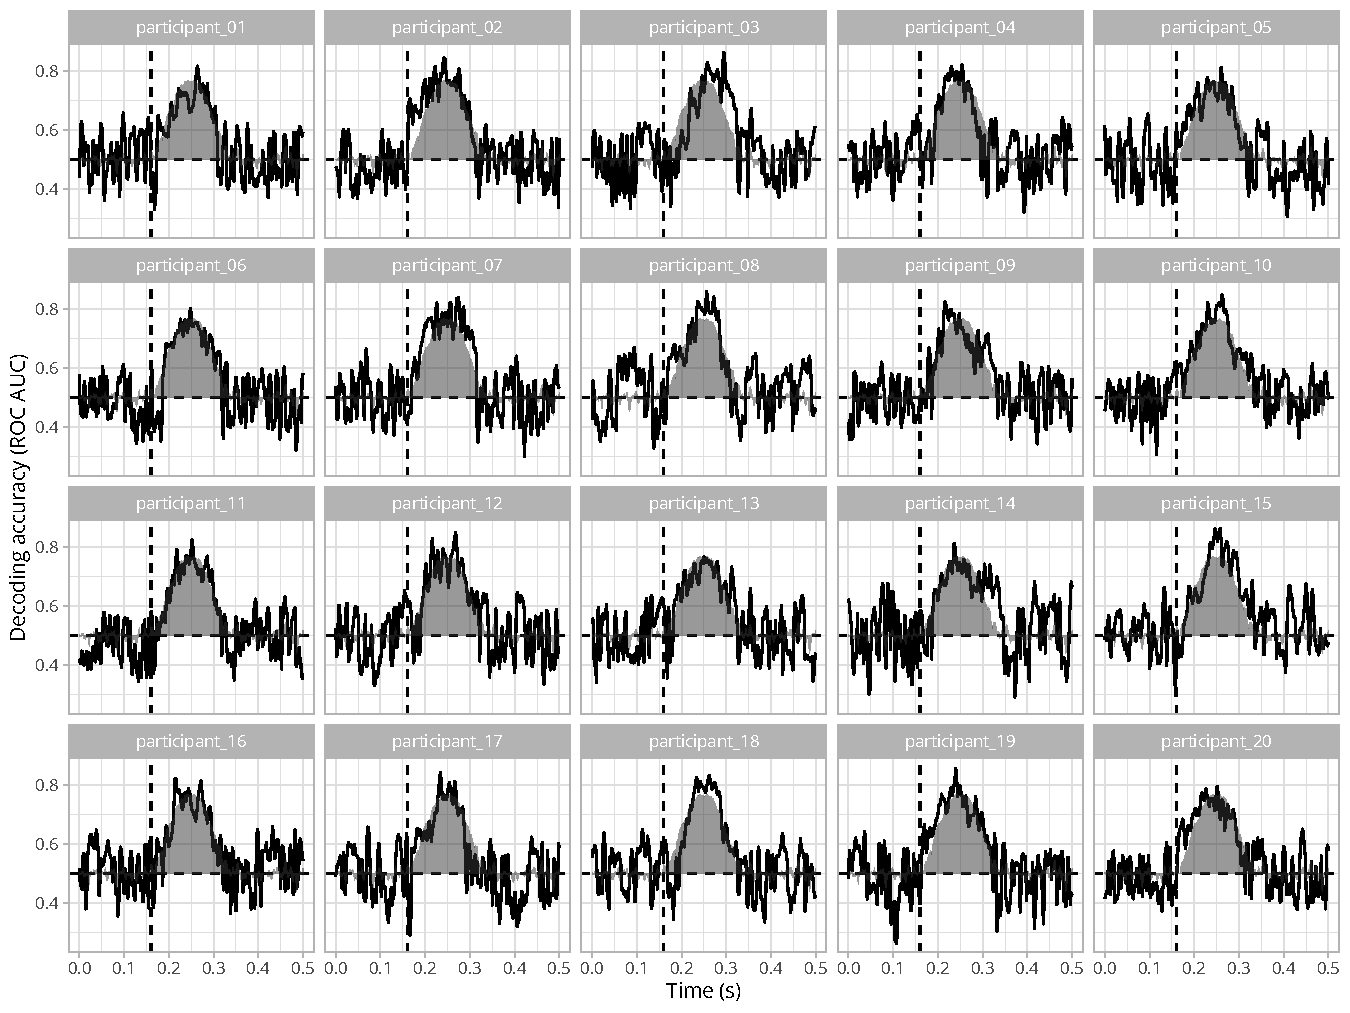
\includegraphics[width=1\textwidth,height=\textheight]{brms_meeg_files/figure-pdf/fig-mne-decoding-1.pdf}

}

\end{figure}%

Now, we want to \emph{test} whether the group-level average decoding
accuracy is above chance (i.e., 0.5) at each timestep. We use a similar
GAM/GP as previously, but we replace the \(\mathrm{Normal}\) likelihood
function by a \(\mathrm{Beta}\) one to account for the bounded nature of
AUC values (between 0 and 1).

\begin{Shaded}
\begin{Highlighting}[]
\CommentTok{\# fitting the GAM}
\NormalTok{decoding\_gam }\OtherTok{\textless{}{-}} \FunctionTok{brm}\NormalTok{(}
\NormalTok{    auc }\SpecialCharTok{\textasciitilde{}} \FunctionTok{s}\NormalTok{(time, }\AttributeTok{bs =} \StringTok{"cr"}\NormalTok{, }\AttributeTok{k =} \DecValTok{10}\NormalTok{),}
    \AttributeTok{data =}\NormalTok{ decoding\_data,}
    \AttributeTok{family =} \FunctionTok{Beta}\NormalTok{(),}
    \AttributeTok{iter =} \DecValTok{5000}\NormalTok{,}
    \AttributeTok{chains =} \DecValTok{4}\NormalTok{,}
    \AttributeTok{cores =} \DecValTok{4}\NormalTok{,}
    \AttributeTok{file =} \StringTok{"models/decoding\_gam.rds"}
\NormalTok{    )}
\end{Highlighting}
\end{Shaded}

\begin{Shaded}
\begin{Highlighting}[]
\CommentTok{\# fitting the GP}
\NormalTok{decoding\_gp }\OtherTok{\textless{}{-}} \FunctionTok{brm}\NormalTok{(}
\NormalTok{    auc }\SpecialCharTok{\textasciitilde{}} \FunctionTok{gp}\NormalTok{(time, }\AttributeTok{k =} \DecValTok{20}\NormalTok{),}
    \AttributeTok{data =}\NormalTok{ decoding\_data,}
    \AttributeTok{family =} \FunctionTok{Beta}\NormalTok{(),}
    \AttributeTok{control =} \FunctionTok{list}\NormalTok{(}\AttributeTok{adapt\_delta =} \FloatTok{0.99}\NormalTok{),}
    \AttributeTok{iter =} \DecValTok{5000}\NormalTok{,}
    \AttributeTok{chains =} \DecValTok{4}\NormalTok{,}
    \AttributeTok{cores =} \DecValTok{4}\NormalTok{,}
    \AttributeTok{file =} \StringTok{"models/decoding\_gp.rds"}
\NormalTok{    )}
\end{Highlighting}
\end{Shaded}

\begin{figure}[H]

\caption{Posterior predictions of the GAM (left) and GP (right) fitted
on decoding accuracy over time.}

{\centering 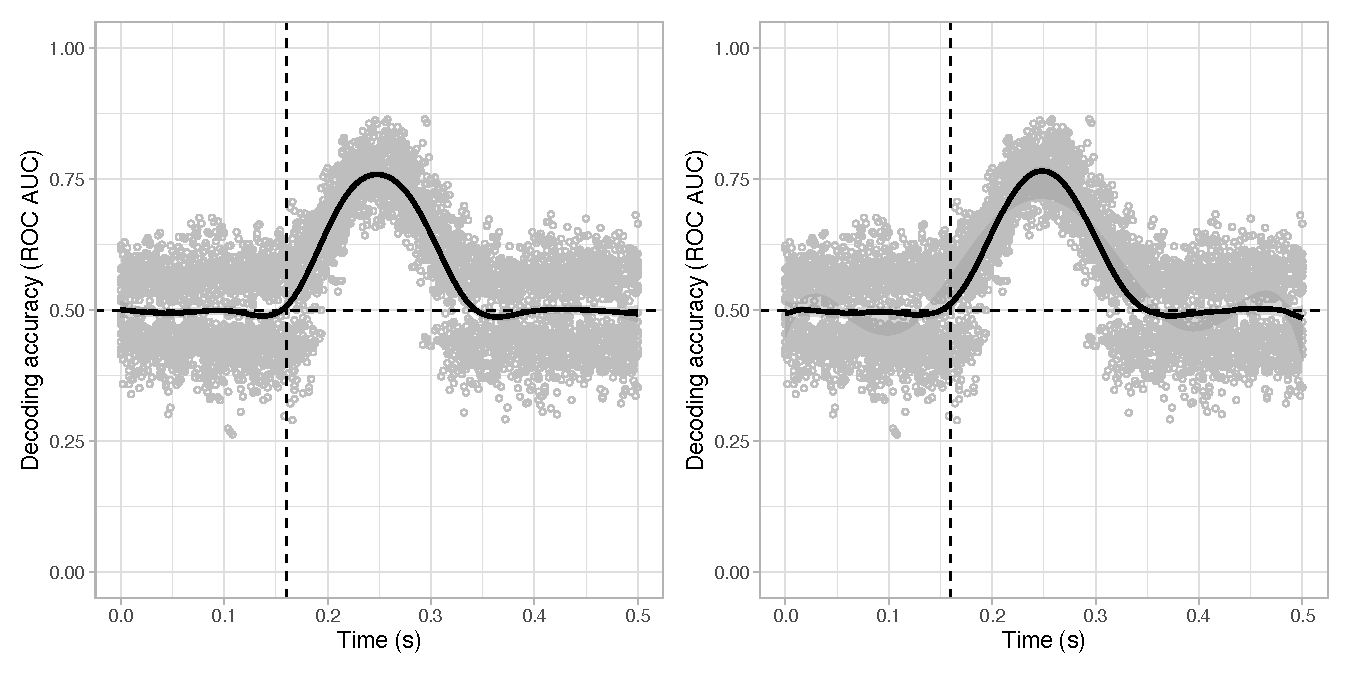
\includegraphics[width=1\textwidth,height=\textheight]{brms_meeg_files/figure-pdf/decoding-preds-1.pdf}

}

\end{figure}%

Next, we plot the posterior probability of decoding accuracy being above
chance level (plus some epsilon) (Figure~\ref{fig-decoding-post}).

\begin{figure}[!htb]

\caption{\label{fig-decoding-post}Posterior probability of decoding
accuracy being above chance level according to the GAM (left) or the GP
(right).}

\centering{

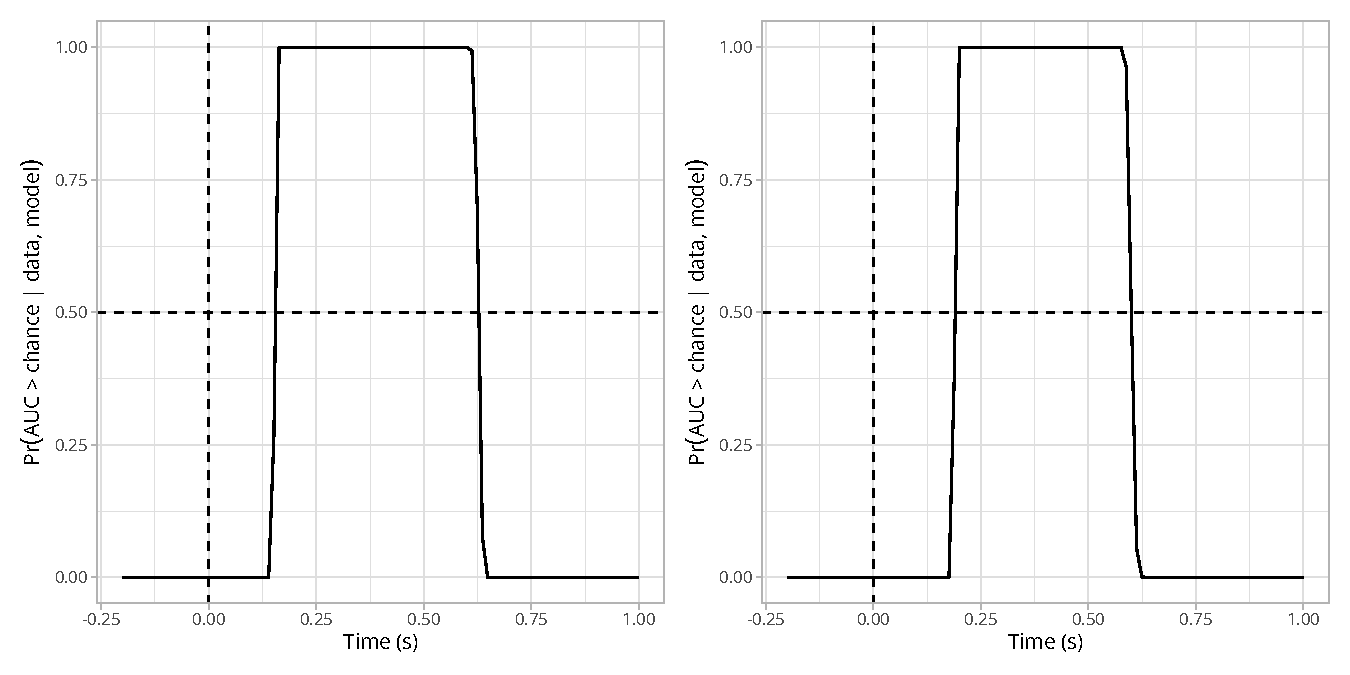
\includegraphics[width=1\textwidth,height=\textheight]{brms_meeg_files/figure-pdf/fig-decoding-post-1.pdf}

}

\end{figure}%

\begin{figure}[!htb]

\caption{\label{fig-decoding-ratio}Ratio of posterior probabilities of
decoding accuracy being above chance level according to the GAM (left)
or the GP (right).}

\centering{

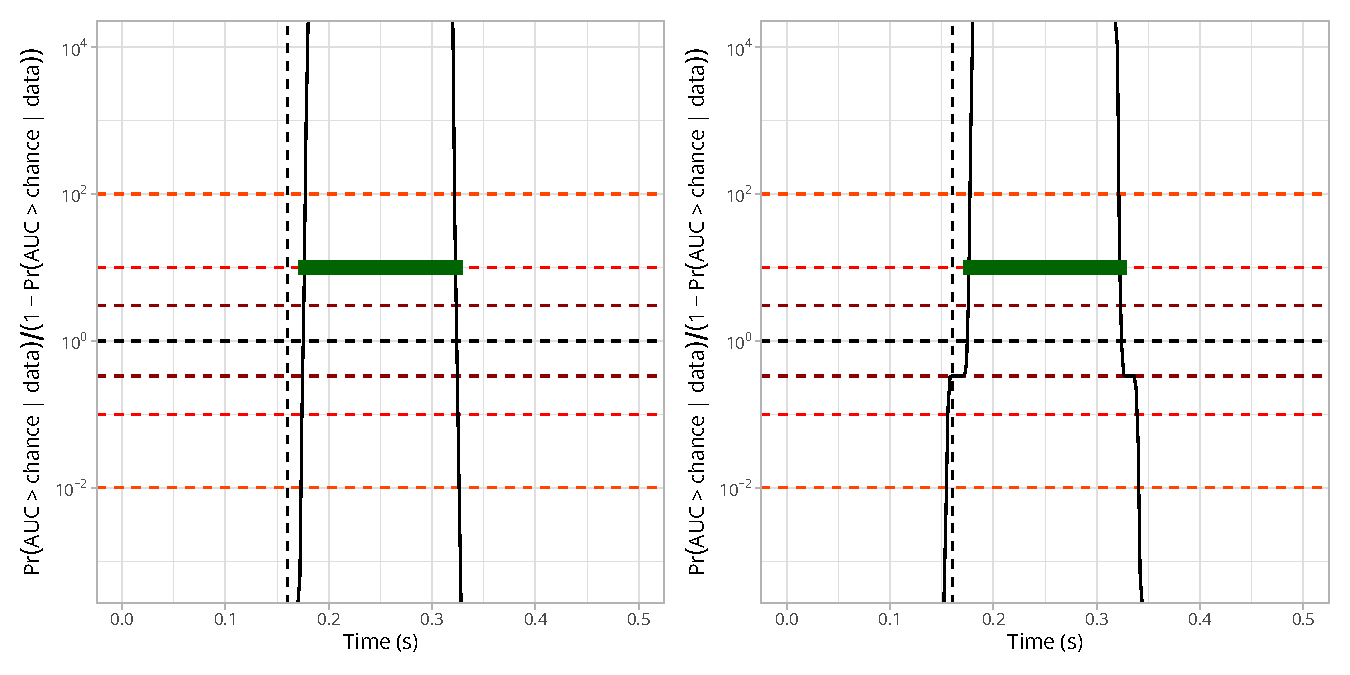
\includegraphics[width=1\textwidth,height=\textheight]{brms_meeg_files/figure-pdf/fig-decoding-ratio-1.pdf}

}

\end{figure}%

\newpage

\section{Application to 2D time-resolved decoding results
(cross-temporal
generalisation)}\label{application-to-2d-time-resolved-decoding-results-cross-temporal-generalisation}

Assume we have M/EEG data and we have conducted cross-temporal
generalisation analyses (\citeproc{ref-king2014}{King \& Dehaene,
2014}). As a result, we have a 2D matrix where each element contains the
decoding accuracy (e.g., ROC AUC) of a classifier trained at timestep
\(\text{training}_{i}\) and tested at timestep \(\text{testing}_{j}\)
(Figure~\ref{fig-sim-timegen}).

\begin{figure}[!htb]

\caption{\label{fig-sim-timegen}Exemplary (simulated) group-level
average cross-temporal generalisation matrix of decoding performance
(ROC AUC).}

\centering{

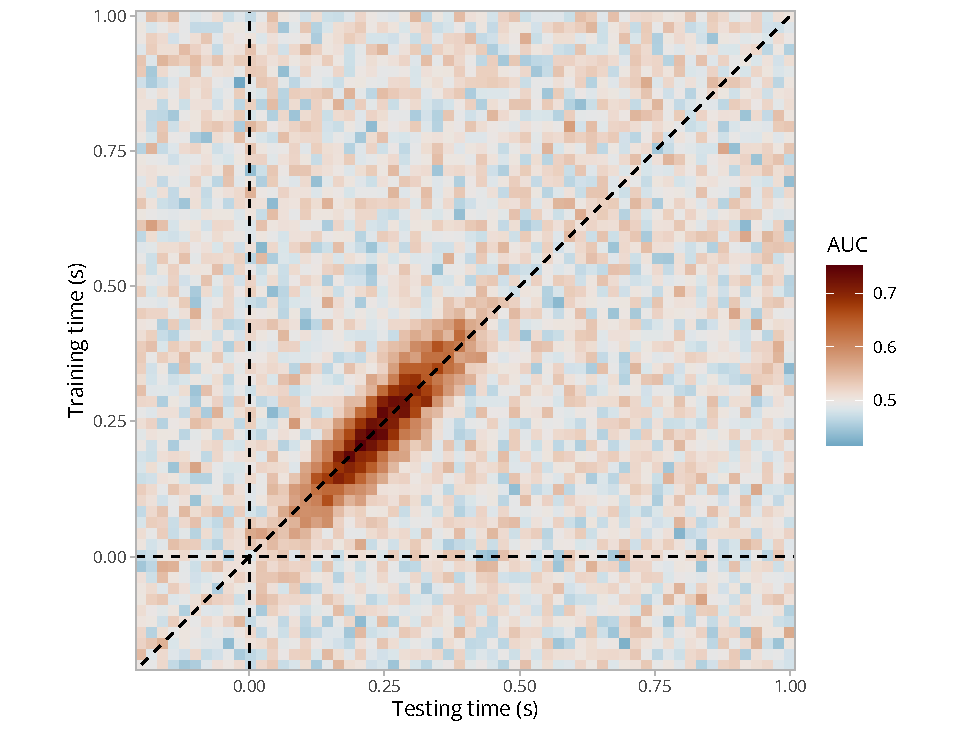
\includegraphics[width=1\textwidth,height=\textheight]{brms_meeg_files/figure-pdf/fig-sim-timegen-1.pdf}

}

\end{figure}%

Now, we want to test whether and when decoding performance is above
chance level (0.5 for a binary decoding task). These two models are
computationally heavier to fit (more observations and 2D smooth
functions)\ldots{}

\begin{Shaded}
\begin{Highlighting}[]
\CommentTok{\# fitting a GAM with two temporal dimensions}
\NormalTok{timegen\_gam }\OtherTok{\textless{}{-}} \FunctionTok{brm}\NormalTok{(}
    \CommentTok{\# 2D thin{-}plate spline (tp)}
    \CommentTok{\# auc \textasciitilde{} s(train\_time, test\_time, bs = "tp", k = 10),}
\NormalTok{    auc }\SpecialCharTok{\textasciitilde{}} \FunctionTok{t2}\NormalTok{(train\_time, test\_time, }\AttributeTok{bs =} \StringTok{"tp"}\NormalTok{, }\AttributeTok{k =} \DecValTok{10}\NormalTok{),}
    \AttributeTok{data =}\NormalTok{ timegen\_data,}
    \AttributeTok{family =} \FunctionTok{Beta}\NormalTok{(),}
    \AttributeTok{iter =} \DecValTok{5000}\NormalTok{,}
    \AttributeTok{chains =} \DecValTok{4}\NormalTok{,}
    \AttributeTok{cores =} \DecValTok{4}\NormalTok{,}
    \AttributeTok{file =} \StringTok{"models/timegen\_gam\_t2.rds"}
\NormalTok{    )}

\CommentTok{\# fitting a GP with two temporal dimensions}
\CommentTok{\# timegen\_gp \textless{}{-} brm(}
\CommentTok{\#     auc \textasciitilde{} gp(train\_time, test\_time, k = 20),}
\CommentTok{\#     data = timegen\_data,}
\CommentTok{\#     family = Beta(),}
\CommentTok{\#     control = list(adapt\_delta = 0.95),}
\CommentTok{\#     iter = 2000,}
\CommentTok{\#     chains = 4,}
\CommentTok{\#     cores = 4,}
\CommentTok{\#     file = "models/timegen\_gp.rds"}
\CommentTok{\#     )}
\end{Highlighting}
\end{Shaded}

\begin{figure}[H]

\caption{Posterior probability of decoding accuracy being above chance
level (2D GAM).}

{\centering 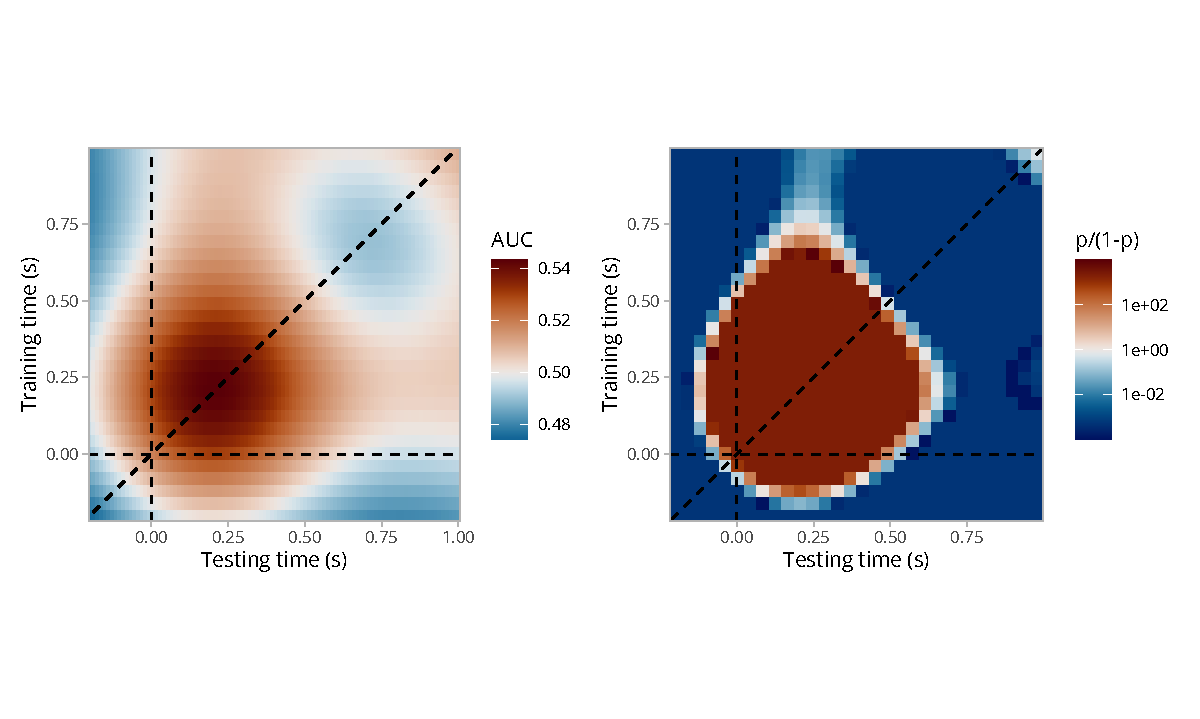
\includegraphics[width=1\textwidth,height=\textheight]{brms_meeg_files/figure-pdf/gam-timegen-post-preds-1.pdf}

}

\end{figure}%

\newpage

\section{Mathematical formulation of the bivariate
GAM}\label{mathematical-formulation-of-the-bivariate-gam}

To model cross-temporal generalisation matrices of decoding performance
(ROC AUC), we extended the initial (decoding) GAM to take into account
the bivariate temporal distribution of AUC values, thus producing
naturally smoothed estimates (timecourses) of AUC values and posterior
probabilities. This model can be written as follows:

\[
\begin{aligned}
\text{AUC}_{i} &\sim \mathrm{Beta}(\mu_{i}, \phi)\\
g(\mu_{i}) &= f \left(\text{train}_{i}, \text{test}_{i} \right)\\
\end{aligned}
\]

where we assume that AUC values come from a \(\mathrm{Beta}\)
distribution with two parameters \(\mu\) and \(\phi\). We can think of
\(f \left(\text{train}_{i}, \text{test}_{i} \right)\) as a surface (a
smooth function of two variables) that we can model using a
2-dimensional splines. Let
\(\mathbf{s}_{i} = \left(\text{train}_{i}, \text{test}_{i} \right)\) be
some pair of training and testing samples, and let
\(\mathbf{k}_{m} = \left(\text{train}_{m}, \text{test}_{m} \right)\)
denote the \(m^{\text{th}}\) knot in the domain of \(\text{train}_{i}\)
and \(\text{test}_{i}\). We can then express the smooth function as:

\[
f \left(\text{train}_{i}, \text{test}_{i} \right) = \alpha + \sum_{m=1}^M \beta_{m} b_{m} \left(\tilde{s}_{i}, \tilde{k}_{m} \right)
\]

Note that \(b_{m}(,)\) is a basis function that maps
\(R \times R \rightarrow R\). A popular bivariate basis function uses
\emph{thin-plate splines}, which extend to
\(\mathbf{s}_{i} \in \mathbb{R}^{d}\) and \(\partial l_{g}\) penalties.
These splines are designed to interpolate and approximate smooth
surfaces over two dimensions (hence the ``bivariate'' term). For \(d=2\)
dimensions and \(l=2\) (smoothness penalty involving second order
derivative):

\[
f \left(\tilde{s}_{i} \right) = \alpha + \beta_{1} x_{i} + \beta_{2} z_{i} +\sum_{m=1}^{M} \beta_{2+m} b_m\left(\tilde{s}_i, \tilde{k}_m\right)
\]

using the the radial basis function given by:

\[
b_m\left(\tilde{s}_i, \tilde{k}_m\right)=\left\|\tilde{s}_i-\tilde{k}_m\right\|^2 \log \left\|\tilde{s}_i-\tilde{k}_m\right\|
\]

where \(\left\|\mathbf{s}_i-\mathbf{k}_{m}\right\|\) is the Euclidean
distance between the covariate \(\mathbf{s}_{i}\) and the knot location
\(\mathbf{k}_{m}\).

\newpage

\section{Threshold-free cluster
enhancement}\label{threshold-free-cluster-enhancement}

Cluster-based permutation approaches require defining a cluster-forming
threshold (e.g., a t- or f-value) as the initial step of the algorithm.
As different cluster-forming thresholds lead to clusters with different
spatial or temporal extent, this threshold modulates the sensitivity of
the subsequent permutation test. The threshold-free cluster enhancement
method (TFCE) was introduced by Smith \& Nichols
(\citeproc{ref-smith2009}{2009}) to overcome this arbitrary threshold.

In brief, the TFCE method works as follows. Instead of picking an
arbitrary cluster-forming threshold (e.g., \(t=2\)), we try all (or
many) possible thresholds in a given range and check whether a given
timestep/voxel belongs to a significant cluster under any of the set of
thresholds\ldots{} Then, instead of using cluster mass, we use a
weighted average between the cluster extend (\(e\), how broad is the
cluster, that is, how many connected samples it contains) and the
cluster height (\(h\), how high is the cluster, that is, how large is
the test statistic) according to the formula:

\[
\text{TFCE} = \int_{h} e(h)^{E} h^{H} \mathrm{d}h
\]

Where\ldots{} the parameters \(E\) and \(H\) are set a priori and
control the influence of the extend and height on the TFCE. Then,
p-value for timestep/voxel \(i\) is computed by comparing it TFCE with
the null distribution of TFCE values. For each permuted signal, we keep
the maximal value over the whole signal for the null distribution of the
TFCE\ldots. But see Sassenhagen \& Draschkow
(\citeproc{ref-sassenhagen2019}{2019})\ldots{}

\newpage

\section{\texorpdfstring{Using the \texttt{R} package and integration
with
\texttt{MNE-Python}}{Using the R package and integration with MNE-Python}}\label{using-the-r-package-and-integration-with-mne-python}

Explain how to use the \texttt{R} package and to integrate it with
\texttt{MNE} epochs\ldots{}

\begin{Shaded}
\begin{Highlighting}[]
\CommentTok{\# to{-}do adding some code here...}
\end{Highlighting}
\end{Shaded}







\end{document}
